% 导言区,进行全局设置
%\documentclass[oneside, 12pt, twocolumn]{ctexbook}%book, report, latter, 引入文档类
\documentclass[oneside, 12pt]{ctexbook}

%\usepackage{ctex}
%\usepackage[fleqn]{amsmath}
\usepackage{amsmath}
\usepackage{amssymb}
\usepackage{fancyhdr}
\usepackage{lastpage}
\usepackage{graphicx}
\usepackage{float}
\usepackage{enumerate} % when need define format to number by myself
\usepackage[colorlinks,linkcolor=black]{hyperref} % set super link
\usepackage{color} % set text color
\usepackage{subfigure} % set two picture on one line

\usepackage{geometry}
\geometry{a4paper,top=2.54cm,left=3.18cm,bottom=2.54cm,right=3.18cm,includehead,includefoot}

% \newcommand命令的定义,新的命令
\newcommand\degree{^\circ}
\title{\kaishu Support Vector Machine}
\author{Fish}
\date{\today}

\graphicspath{{figures/}} %图片在当前目录下的figures目录

% 内容与格式分离
% 设置标题的格式
\ctexset {
	section = {
		format+=\zihao {-4} \heiti \raggedright,
		%name = {,},
		%number = \chinese{section},
		beforeskip = 1.0ex plus 0.2ex minus .2ex,
		afterskip = 1.0ex plus 0.2ex minus .2ex,
		aftername = \hspace{0pt}
	},
	subsection = {
		format+=\zihao{5} \heiti \raggedright,
		% name={\thesubsection},
		name = {,},
		%number = \arabic{subsection},
		beforeskip = 1.0ex plus 0.2ex minus .2ex,
		afterskip = 1.0ex plus 0.2ex minus .2ex,
		aftername = \hspace{0pt}
	}
}


% 正文区(文稿区),有且只有一个document环境
% \begim{*环境名称}
%        内容
% \end{*环境名称}
\begin{document}
	\maketitle
	%\clearpage
	\cleardoublepage
	\thispagestyle{empty}
	\renewcommand{\contentsname}{Content} % set the 目录 to Content
	\tableofcontents
	\thispagestyle{plain}
	
	\clearpage
	\pagestyle{fancy}
	\lhead{Support Vector Machine by wzs}                   
	\rhead{Page \thepage{} of \pageref{LastPage}}
	\setcounter{page}{1}
	
	\chapter{\quad perception}
		\thispagestyle{fancy}
		\section{\quad concept}
			\begin{enumerate}
				\item 感知机是二类分类的线性分类模型, 其输入空间为实例的特征向量, 输出为实例的类别, 取+1和-1二值.
				
				\item 感知机对应于输入控件((特征空间) 中将实例划分为正负两类的分离超平面, 是一种线性分类模型, 属于判别模型. 
				
				\item 感知机学习旨在求出将训练数据进行线性划分的分离超平面.
				
				\item 导入基于误分类的损失函数, 利用梯度下降法对损失函数进行极小化, 求得感知机模型.
				
				\item $f(x) = sign(w \cdot x + b)$
			\end{enumerate}
		
		\section{\quad linearly separable dataset}
			给定数据集$T = \{ (x_1, y_1), (x_2, y_2), ..., (x_N, y_N)\}$,
			其中, $x_i \in \chi = \boldsymbol{\text{R}}^n$, $y_i \in \gamma = \{ +1, -1\}$, $ i = 1,2,...,N$.
			
			如果存在某个超平面S: $w \cdot x + b = 0$ 
			将数据集的正负实例点完全正确划分到超平面的两侧:
			
			对所有 $y_i = +1$ 的实例 $i$, 有 $w \cdot x_i + b > 0$
			
			对所有 $y_i = -1$ 的实例 $i$, 有 $w \cdot x_i + b < 0$
			
			则数据集 $T$ 为线性数据可分数据集, 否则称 数据集 $T$ 线性不可分
	
		\section{\quad loss function}
			假设训练数据集是线性可分的, 为了找出可将训练集正负实例点完全正确分开的分离超平面, 即确定参数 $w, b$, 需要确定一个学习策略, 即定义 (经验) 损失函数并将损失函数极小化 
			
			两种选择:
			\begin{enumerate}
				\item 选择误分类点的总数, 但这样的损失函数不是参数 $w, b$ 的连续可导函数, 不易优化
				
				\item 选择误分类点到超平面S的总距离
			\end{enumerate}
		
			定义输入空间 $\boldsymbol{\text{R}}^n$ 中任一点 $x_0$ 到超平面 $S$ 的距离:
				\begin{align}
					\frac{1}{\parallel w \parallel} |w \cdot x_0 + b|
				\end{align}
			这里 $\parallel w \parallel$ 是 $w$ 的 $L_2$ 范数.
			
			对于误分类的数据 $(x_i, y_i)$ 来说:
				\begin{align}
					-y_i(w \cdot w_i + b) > 0
				\end{align}
			成立. 
			
			因此, 误分类点 $x_i$ 到超平面 $S$ 的距离是
				\begin{align}
					-\frac{1}{\parallel w \parallel} y_i (w \cdot x_i + b)
				\end{align}
			
			这样, 假设超平面 $S$ 的误分类点集合为 $M$, 则所有误分类点到超平面 $S$ 的总距离为 
				\begin{align}
					-\frac{1}{\parallel w \parallel} \sum_{x_i \in M} y_i (w \cdot x_i + b)
				\end{align}
				
			不考虑 $\frac{1}{\parallel w \parallel}$, 得到感知机 $sign(w \cdot x + b)$ 在训练集 $T$ 的损失函数定义为
				\begin{align}
					L(w, b) = -\sum_{x_i \in M} y_i (w \cdot x_i + b)
				\end{align}
				
		\section{\quad original form of perception algorithm}
			关键: 感知机算法是误分类驱动的, 当误分类点位于分离超平面的错误一侧时, 调整 $w, b$ 的值, 使分离超平面向该误分类点的一侧移动, 以减少该误分类点与超平面间的距离, 直至超平面越过该误分类点使其被正确分类.\\
			
			输入: 训练数据集 $T = \{ (x_1, y_1), (x_2, y_2), ..., (x_N, y_N)\}$,
			其中, $x_i \in \chi = \boldsymbol{\text{R}}^n$, $y_i \in \gamma = \{ +1, -1\}$, $ i = 1,2,...,N; \ \text{学习率} \ \eta \ (0 < \eta \leq 1)$.
			
			输出: $w, b$; 感知机模型 $f(x) = sign(w \cdot x + b)$.
				\begin{enumerate}
					\item 选取初值 $w_0, b_0$
					
					\item 在训练集中选取数据 $(x_i, y_i)$
					
					\item 如果 $y_i (w_i + b) \leq 0$
						\begin{enumerate}
							\item 损失函极小化 $\underset{w,b}{\min}L(w, b) = -\sum\limits_{x_i \in M} y_i (w \cdot x_i + b)$
							
							\item 梯度
								\begin{align}
									\nabla_w L(w, b) &= -\sum_{x_i \in M} y_i x_i \\
									\nabla_b L(w, b) &= -\sum_{x_i \in M} y_i
								\end{align}
								
							\item 随机选取一个误分类点 $(x_i, y_i)$, 更新参数 $w, b$
								\begin{align}
									w &\leftarrow w + \eta y_i x_i \\
									b &\leftarrow b + \eta y_i
								\end{align}
						\end{enumerate}
					
					\item 转至 (2), 直至训练集中没有误分类点。
			\end{enumerate}
			
		\section{\quad dual form of perception algorithm}
			基本思路: 将 $w$ 和 $b$ 表示为实例 $x_i$ 和标记 $y_i$ 的线性组合的形式, 通过求解其系数而求得 $w$ 和 $b$. 
			
			输入: 训练数据集 $T = \{ (x_1, y_1), (x_2, y_2), ..., (x_N, y_N)\}$,
			其中, $x_i \in \chi = \boldsymbol{\text{R}}^n$, $y_i \in \gamma = \{ +1, -1\}$, $ i = 1,2,...,N; \ \text{学习率} \ \eta \ (0 < \eta \leq 1)$.
			
			输出: $\alpha, b$; 感知机模型 $f(x) = sign \left( \sum\limits_{j=1}^{N} \alpha_j y_j x_j \cdot x + b \right) $
			
			其中, $\alpha = (\alpha_1, \alpha_2, ..., \alpha_N)^T$ , 注意这里是一个向量, 所以后面更新时, $\alpha$ 直接定义步长更新
			
			\begin{enumerate}
				\item $\alpha \leftarrow 0, b \leftarrow 0$
				
				\item 在训练集中选取数据 $(x_i, y_i)$
				
				\item 如果 $y_i \left( \sum\limits_{j=1}^{N} \alpha_j y_j x_j \cdot x_i + b \right)$
					\begin{enumerate}
						\item 损失函极小化 $\underset{w,b}{\min}L(w, b) = \underset{\alpha,b}{\min}L(\alpha, b) = -\sum\limits_{x_i \in M} y_i (\alpha_j y_j x_j \cdot x_i + b)$
						
						\item 梯度
						\begin{align}
						\nabla_b L(w, b) &= -\sum_{x_i \in M} y_i
						\end{align}
						
						\item 随机选取一个误分类点 $(x_i, y_i)$, 更新参数 $w, b$
						\begin{align}
						\alpha &\leftarrow \alpha + \eta \\
						b &\leftarrow b + \eta y_i
						\end{align}
					\end{enumerate}
				
				\item 转至 (2) 直到没有误分类数据.
			\end{enumerate}
			
			注意: 对偶形式中训练实例仅以内积的形式出现.
			
			为了方便, 预先将训练集中实例间的内积计算出来并以矩阵的形式存储,即 Gram 矩阵
			\begin{equation}
				G = \left[ x_i \cdot x_j \right]
			\end{equation}
		
	\chapter{\quad Convex function}
		\thispagestyle{fancy}
		\section{\quad Convex collection and Convex function}
			\subsection{\quad Convex function}
				$y = x^2$ 是凸函数, 函数图像上位于 $y = x^2$ 上方的区域构成凸集.
				\begin{enumerate}
					\item 凸函数图像的上方区域, 一定是凸集
							
					\item 一个函数图像的上方区域为凸集, 则该函数是凸函数
				\end{enumerate}
		
			\subsection{\quad Convex collection}
				\begin{enumerate}
					\item Afiine set 仿射集
						\begin{enumerate}
							\item define: 通过集合 C 中任意两个不同点的直线仍然在集合 C 内, 则称集合 C 为仿射集.
							 	\begin{align}
							 		\forall x_1, x_2 \in C, \forall \theta \in R, \ \text{则} \ x = \theta \cdot x_1 + (1 - \theta) \cdot x_2 \in C
							 	\end{align}
							 	
							 \item 仿射集的例子: 直线、平面、超平面
							 
							 	$n$ 维空间的 $n-1$ 维仿射集为 $n-1$维超平面
						\end{enumerate}
					
					\item Convex 凸集\\
						两种表述 (可以思考其内涵一样吗) :
						\begin{enumerate}
							\item 集合 C 内任意两点间的线段均在集合 C 内, 则称集合 C 为凸集.
								\begin{align}
									\forall x_1, x_2 \in C, \forall \theta \in \left[ 0, 1 \right], \ \text{则} \ x = \theta \cdot x_1 + (1 - \theta) \cdot x_2 \in C
								\end{align}
								
							\item k个点的版本:
								\begin{align}
									\forall x_1, x_2, ..., x_k \in C, \theta_i \in [0,1] \text{且} \sum_{i=1}^{k} \theta_i x_i \in C
								\end{align}
						\end{enumerate}
					
					\item 因为仿射集的条件比凸集的条件强, 所以, 仿射集必然是凸集
					
					\item judgement of convex collection 	
						\begin{figure}[H]
							\vspace{-0.2cm}  %调整图片与上文的垂直距离
							\setlength{\abovecaptionskip}{-0.2cm}   %调整图片标题与图距离
							%\setlength{\belowcaptionskip}{-1cm}   %调整图片标题与下文距离
							\centering
							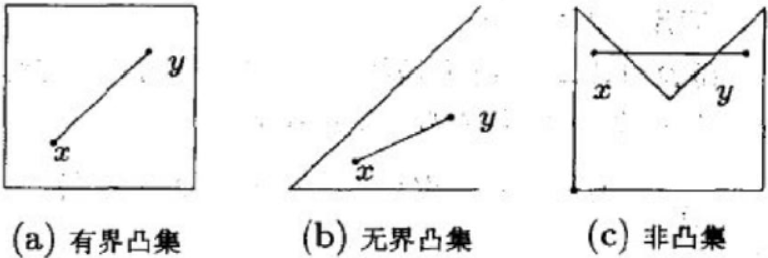
\includegraphics[scale=0.6]{convex_collection.png}
							\renewcommand{\figurename}{Fig} % set picture title starting with Fig or 图
							\caption{convex collection}
							\label{fig:1}
						\end{figure}
				\end{enumerate}
			
		\section{\quad affine transformation}
			\subsection{\quad concept}
				函数 $f(x) = Ax + b$ 的形式, 称函数是放射的: 即线性函数加常数的形式
				
			\subsection{\quad theory}
				\begin{enumerate}
					\item 仿射变换 $f(x) = Ax + b$, $A \in \boldsymbol{\text{R}}^{m \times n}$, $b \in \boldsymbol{\text{R}}^m$
						\begin{enumerate}
							\item 伸缩、平移、投影
						\end{enumerate}
					
					\item 若 $f$ 是仿射变换, $f : \boldsymbol{\text{R}}^n \rightarrow \boldsymbol{\text{R}}^m \ \quad f(S) = \{ f(x) | x \in S \}$
						\begin{enumerate}
							\item 若 $S$ 为凸集, 则 $f(x)$ 为凸集;
							
							\item 若 $f(S)$ 为凸集, 则 $S$ 为凸集. 
						\end{enumerate}
					
					\item 两个凸集的和为凸集
						\begin{align}
							S_1 + S_2 = \{ x + y | x \in S_1, y \in S_2 \}
						\end{align}
						
					\item 两个凸集的笛卡尔积 (直积) 为凸集
						\begin{align}
							S_1 \times S_2 = \{ (x_1, x_2) | x \in S_1, x_2 \in S_2 \}
						\end{align}
						
					\item 两个集合的部分和为凸集 (分配率)
						\begin{align}
							S = \{ (x, y_1 + y_2) | (x, y_1) \in S_1, (x, y_2) \in S_2 \}
						\end{align}
				\end{enumerate}
			
		\section{\quad perspective collineation}
			\subsection{\quad concept}
				透视函数对向量进行伸缩 (规范化), 使得最后一维的分量为 1 并舍弃之.
					\begin{align}
						P : \boldsymbol{\text{R}}^{n+1} \rightarrow \boldsymbol{\text{R}}^{n}, \ P(z, t) = z/t
					\end{align}
			
			\subsection{\quad direct significance}
				小孔成像
				\begin{figure}[H]
					\vspace{-0.2cm}  %调整图片与上文的垂直距离
					\setlength{\abovecaptionskip}{-0.2cm}   %调整图片标题与图距离
					%\setlength{\belowcaptionskip}{-1cm}   %调整图片标题与下文距离
					\centering
					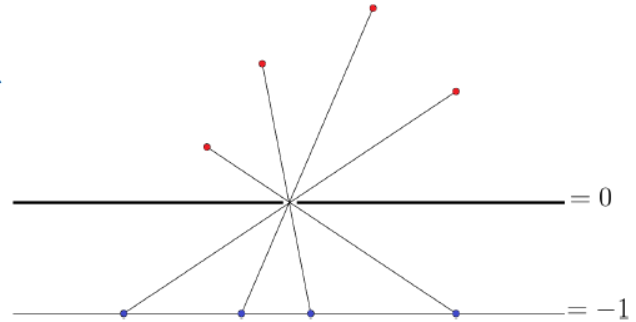
\includegraphics[scale=0.6]{perspective_collineation.png}
					\renewcommand{\figurename}{Fig} % set picture title starting with Fig or 图
					\caption{significance of perspective collineation}
					\label{fig:2}
				\end{figure}
			
			\subsection{\quad summary}
				凸集的透视变换仍然是凸集
				
		\section{\quad segmentation plane}
			\subsection{\quad concept}
				设 C 和 D 为两不相交的凸集, 则存在超平面 P, P可以将 C 和 D 分离.
				\begin{align}
					\forall x \in C, a^T x \leq b \ \text{且} \ \forall x \in D, a^T x \geq b
				\end{align}
				
			\subsection{\quad segmentation plane}
				\begin{figure}[H]
					\vspace{-0.2cm}  %调整图片与上文的垂直距离
					\setlength{\abovecaptionskip}{-0.2cm}   %调整图片标题与图距离
					%\setlength{\belowcaptionskip}{-1cm}   %调整图片标题与下文距离
					\centering
					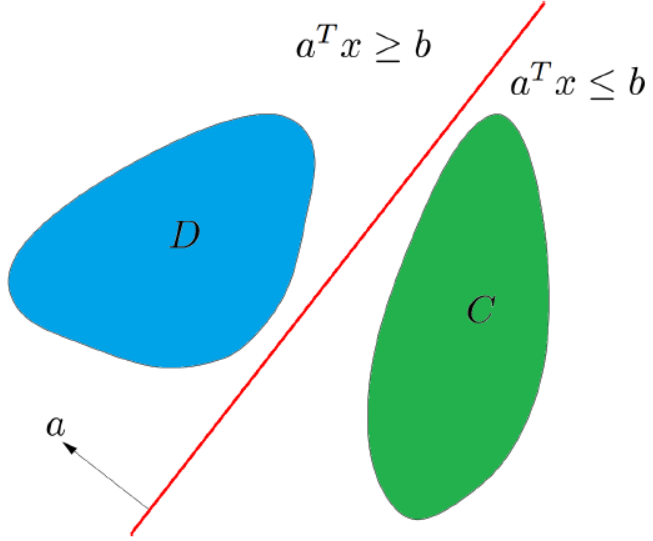
\includegraphics[scale=0.6]{segmentation_plane.png}
					\renewcommand{\figurename}{Fig} % set picture title starting with Fig or 图
					\caption{segmentation plane}
					\label{fig:3}
				\end{figure}
			
			\subsection{\quad the structure of sefmentation plane}
				\begin{enumerate}
					\item 两个集合的距离, 定义为两个集合间元素的最短距离
					
					\item 做集合 C 和集合 D 最短线段的垂直平分线
					
					\item picture
						\begin{figure}[H]
							\vspace{-0.2cm}  %调整图片与上文的垂直距离
							\setlength{\abovecaptionskip}{-0.2cm}   %调整图片标题与图距离
							%\setlength{\belowcaptionskip}{-1cm}   %调整图片标题与下文距离
							\centering
							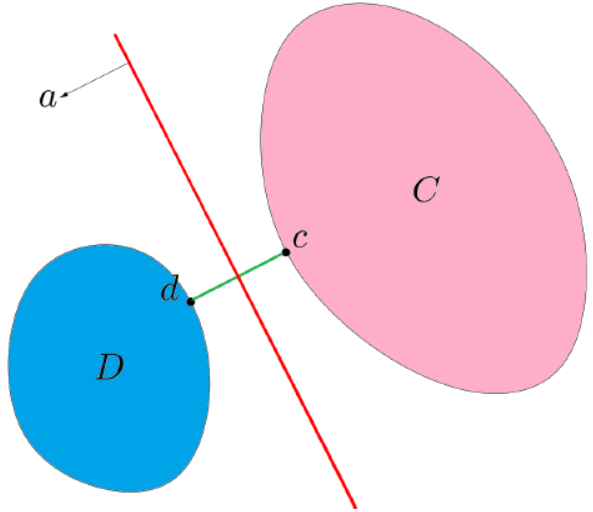
\includegraphics[scale=0.5]{the_distance_of_segmentation.png}
							\renewcommand{\figurename}{Fig} % set picture title starting with Fig or 图
							\caption{the distance of segmentation plane}
							\label{fig:4}
						\end{figure}
				\end{enumerate}
			
			\subsection{\quad support hyperplane}
				\begin{figure}[H]
					\vspace{-0.2cm}  %调整图片与上文的垂直距离
					\setlength{\abovecaptionskip}{-0.2cm}   %调整图片标题与图距离
					%\setlength{\belowcaptionskip}{-1cm}   %调整图片标题与下文距离
					\centering
					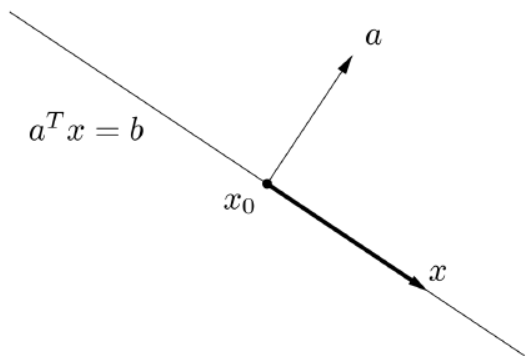
\includegraphics[scale=0.5]{hyperplane.png}
					\renewcommand{\figurename}{Fig} % set picture title starting with Fig or 图
					\caption{hyperplane}
					\label{fig:5}
				\end{figure}
			
				\begin{enumerate}
					\item 设集合 C , $x_0$ 为 C 边界上的点. 若存在 $a \neq 0$, 满足对任意 $x \in C$, 都有 $a^T x \leq a^T x_0$ 成立, 则称超平面 $\{ x | a^T x = a^T x_0 \}$ 为集合 C 在点 $x_0$ 处的支撑超平面.
					
					\item 凸集边界上任意一点, 均存在支撑超平面
					
					\item 反之, 若在一个闭的非中空 (内部点不为空) 集合, 在边界上的任意一点存在支撑超平面, 则该集合为凸集
				\end{enumerate}
			
			\subsection{\quad question}
				\begin{enumerate}
					\item 如何定义两个集合的 “最优” 分割超平面?
						\begin{enumerate}
							\item 找到集合 “边界” 上的若干点, 以这些点为 “基础” 计算超平面的方向; 以两个集合边界上的这些点的平均作为超平面的 “截距”
							
							\item 支持向量: support vector
							
							\item optimal segmentation plane
								\begin{figure}[H]
									\vspace{-0.2cm}  %调整图片与上文的垂直距离
									\setlength{\abovecaptionskip}{-0.2cm}   %调整图片标题与图距离
									%\setlength{\belowcaptionskip}{-1cm}   %调整图片标题与下文距离
									\centering
									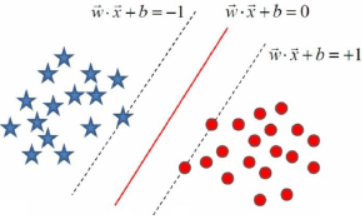
\includegraphics[scale=0.6]{optimal_segmentation_plane.png}
									\renewcommand{\figurename}{Fig} % set picture title starting with Fig or 图
									\caption{optimal segmentation plane}
									\label{fig:6}
								\end{figure}
						\end{enumerate}
					
					\item 若两个集合有部分相交, 如何定义超平面, 使得两个集合 “尽量” 分开?
						\begin{enumerate}
							\item 注: 上述 “集合” 不一定是凸集, 可能是由若干离散点组成. 若一组集合为 $(x, 1)$, 另一组集合为 $(x, 2)$, 则为机器学习中的分类问题.
						\end{enumerate}
				\end{enumerate}
			
		\section{\quad property of convex function}
			\subsection{\quad concept}
				若函数 $fx(x)$ 的定义域 domf 为凸集, 且满足
				\begin{align}
					\forall x, y \in \text{dom} \ f, \ 0 \leq \theta \leq 1, \ \text{有}\\
					f(\theta x + (1-\theta)y) \leq \theta f(x) + (1-\theta)f(y)
				\end{align}
				\begin{figure}[H]
					\vspace{-0.6cm}  %调整图片与上文的垂直距离
					\setlength{\abovecaptionskip}{-0.2cm}   %调整图片标题与图距离
					%\setlength{\belowcaptionskip}{-1cm}   %调整图片标题与下文距离
					\centering
					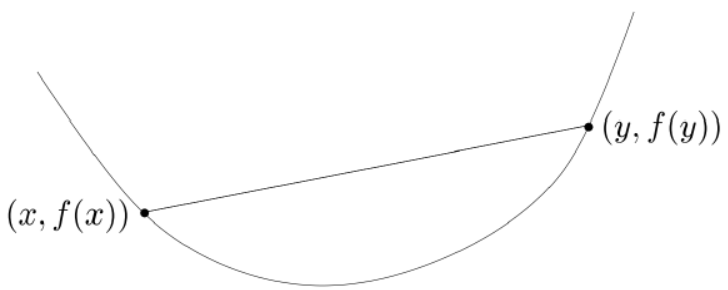
\includegraphics[scale=0.6]{convex_function.png}
					\renewcommand{\figurename}{Fig} % set picture title starting with Fig or 图
					\caption{convex function}
					\label{fig:7}
				\end{figure}
					
			\subsection{\quad first-order derivative of convex function}
				若 $f(x)$ 一阶可微, 则函数 f 为凸函数当前仅当 f 的定义域 domf 为凸集, 且
				\begin{align}
					\forall x, y \in \text{dom} \ f, \ f(y) \geq f(x) + \nabla f(x)^T (y-x)
				\end{align}
				\begin{figure}[H]
					\vspace{-0.6cm}  %调整图片与上文的垂直距离
					\setlength{\abovecaptionskip}{-0.2cm}   %调整图片标题与图距离
					%\setlength{\belowcaptionskip}{-1cm}   %调整图片标题与下文距离
					\centering
					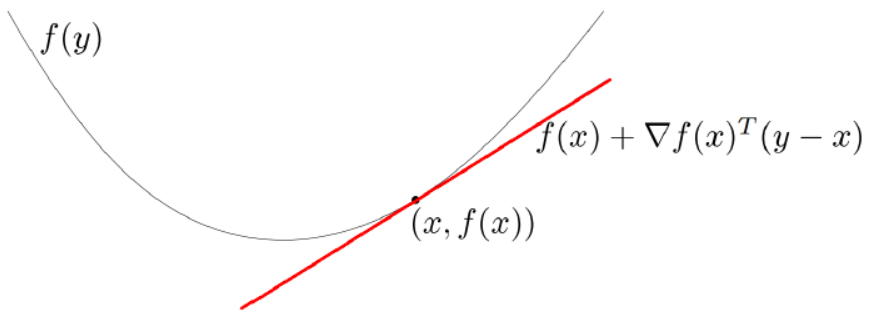
\includegraphics[scale=0.6]{first_derivation_of_convex_function.png}
					\renewcommand{\figurename}{Fig} % set picture title starting with Fig or 图
					\caption{first-order derivative of convex function}
					\label{fig:8}
				\end{figure}
				
				对于凸函数, 其一阶 Taylor 近似本质上是该函数的全局下估计
				
			\subsection{\quad second-order derivative of convex function}
				\begin{enumerate}
					\item 若函数 f 二阶可微, 则函数 f 为凸函数当前仅当 dom 为凸集, 且
						\begin{equation}
							\nabla^2 f(x) \succ = 0
						\end{equation}
						
					\item 若 f 是一元函数, 上式表示二阶导大于等于0
					
					\item 若 f 是多元函数, 上式表示二阶导 Hessian 矩阵半正定
				\end{enumerate}

		\section{\quad examples of convex function}
			\begin{itemize}
				\item 指数函数 $f(x) = e^{ax}$
				
				\item 幂函数 $f(x) = x^a, x \in R^+, a \geq 1 \ \text{或} \ a \leq 0$
				
				\item 负对数函数 $f(x) = -\ln x$
				
				\item 负熵函数 $f(x) = x\ln x$
				
				\item 范数函数 $f(\vec{x}) = \parallel x \parallel$
				
				\item 最大值函数 $f(\vec{x}) = \max (x_1, x_2, ..., x_n)$
				
				\item 指数线性函数 $f(\vec{x}) = \log \left( e^{x_1} + e^{x_2} + ... + e^{x_n} \right)$
			\end{itemize}
			
	\chapter{\quad Convex Optimization}
		\thispagestyle{fancy}
		\section{\quad optimization problem}
			\begin{enumerate}
				\item common format
					\begin{align}
						\begin{split}
						\text{minimize} \ &f_0(x), x \in \boldsymbol{\text{R}}^n \\
						\text{subject to} \ &g_i(x) \leq 0, \ i=1, ..., m \\
						&h_j(x) = 0, \ j=1, ..., p\\
						\text{优化变量} \quad &x \in \boldsymbol{R}^n \\
						\text{不等式约束} \quad &g_i(x) \leq 0\\
						\text{等式约束} \quad &h_j(x) = 0\\
						\text{无约束优化} \quad &m = p = 0	\label{eq:optimization_problem}									
						\end{split}
					\end{align}
					
				\item domain of optimal problem
					\begin{align}
						D = \bigcap\limits_{i=0}^{m} \text{dom} g_i \cap \bigcup\limits_{j=1}^{p} \text{dom} h_j
					\end{align}
					
				\item feasible dot (solution)
					\begin{itemize}
						\item $x \in D$, 满足式 \ref{eq:optimization_problem} 中约束条件
					\end{itemize}
				
				\item feasible domain (feasible collection)
					\begin{itemize}
						\item 所有可行点的集合 
					\end{itemize}
				
				\item optimization value
					\begin{align}
						p^* = \inf \{ f_0(x) | g_i(x) \leq 0, i=1,...,m, h_j(x)=0,j=1,...,p\}
					\end{align}
					
				\item optimization solution
					\begin{align}
						p^* = f_0(x^*)
					\end{align}
			\end{enumerate}
		
		\section{\quad convex optimization}
			\subsection{\quad basic form}
				\begin{align}
					\begin{split}
						\text{minimize} \quad &f_0(x), x \in \boldsymbol{\text{R}}^n \\
						\text{subject to} \quad &g_i(x) \leq 0, i=1,...,m \\
						&h_j(x) = 0, j=1,...,p
					\end{split}
				\end{align}
				\begin{enumerate}
					\item among, $g_i(x)$ 为凸函数, $h_j(x)$ 为仿射函数
					
					\item important property of convex optimization problem
						\begin{enumerate}
							\item 凸优化问题的可行域为凸集
							
							\item 凸优化问题的局部最优解即为 \textcolor{red}{全局最优解}
						\end{enumerate}
				\end{enumerate}
			
			\subsection{\quad Lagrange乘子法}
				在支持向量机模型 (SVM) 的推导中一步很关键的就是利用 Lagrange 对偶性 将原问题转化为对偶问题.
				\begin{enumerate}
					\item theoty: \\
						一般的求极值问题, 求导等于0. 但是如果不但要求极值, 还要求一个满足一定约束条件的极值, 那么此时就可以构造 Lagrange 函数, 其实就是 \textcolor{red}{把约束项添加到原函数上, 然后对构造的新函数求导}
						
					\item example picture
						\begin{figure}[H]
							\vspace{-0.6cm}  %调整图片与上文的垂直距离
							\setlength{\abovecaptionskip}{-0.2cm}   %调整图片标题与图距离
							%\setlength{\belowcaptionskip}{-1cm}   %调整图片标题与下文距离
							\centering
							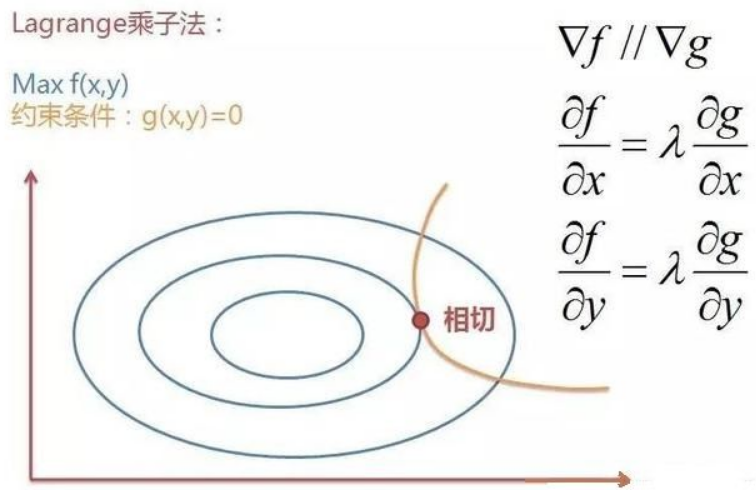
\includegraphics[scale=0.6]{Lagrange_multiplier.png}
							\renewcommand{\figurename}{Fig} % set picture title starting with Fig or 图
							\caption{Lagrange multiplier method}
							\label{fig:9}
						\end{figure}
					
					\item analysis: \\
					对于一个要求极值的函数 $f(x, y)$, 图上的蓝圈就是这个函数的等高图, 就是说 $f(x, y) = c_1, c_2, ..., c_n$ 分别代表不同的数值 (每个值代表一圈, 等高图), 我要找到一组 $(x, y)$, 使它的 $c_i$ 值越大越好, 但是这点必须满足约束条件 $g(x, y)$ (在黄线上)
					
					\item conclusion: \\
					就是说 $f(x, y)$ 和 $g(x, y)$ 相切, 或者说它们的梯度 $\nabla f$ 和 $\nabla g$ 平行, 因此它们的梯度 (偏导) 成倍关系; 那我们就假设为 $\lambda$ 倍, 然后把约束条件加到原函数后再对它求导, 其实就等于满足了图上的式子了.
				\end{enumerate}

					
			
			\subsection{ Lagrange 函数的极小极大最优值 $\min\limits_x\max\limits_{\lambda, \nu: \lambda_i \geq 0} L(x, \lambda, \nu)$ 和 原问题的最优值 $p^*$}
				\begin{enumerate}
					\item 一般优化问题的 Lagrange 乘子法
						\begin{align}
							\begin{split}
								\text{minimize} \quad &f_0(x), x \in \boldsymbol{\text{R}}^n \\
								\text{subject to} \quad &g_i(x) \leq 0, i=1,...,m \\
								&h_j(x) = 0, j=1,...,p
							\end{split}
						\end{align}
						
					\item Lagrange 函数
						\begin{align}
							L(x, \lambda, \nu) = f_0(x) + \sum_{i=1}^{m} \lambda_i g_i(x) + \sum_{j=1}^{p} \nu_j h_j(x) \label{eq2: Lagrange_funtion}
						\end{align}
						对固定的 x, Lagrange 函数 $L(x, \lambda, \nu)$ 为关于 $\lambda$ 和 $\nu$ 的仿射函数, 这里, $x = (x^1, x^2, ..., x^n)^T \in \boldsymbol{\text{R}}^n, \lambda, \nu$ 是	Lagrange 乘子, $\lambda \geq 0$
						
					\item \textcolor{red}{Lagrange 函数的极小极大最优值 $\min\limits_x\max\limits_{\lambda, \nu: \lambda_i \geq 0} L(x, \lambda, \nu)$ 和 原问题的最优值 $p^*$ 之间的关系}
					
					考虑 x 的函数: 
						\begin{align}
							f(x) = \max\limits_{\lambda, \nu : \lambda \geq 0} L (x, \lambda, \nu) \label{eq3: Lagrange and original problem}
						\end{align}
					即\textcolor{red}{原问题 $f(x)$ 与 Lagrange 函数在 乘子变量最大化 时的值是等价的}
					
					\item 证明上式:
					假设给定某个 x, 如果 x 违反原始问题的约束条件, 即存在某个 $i$ 使得 $g_i(x) > 0$ 或者存在某个 $j$ 使得 $h_j(x) \neq 0$, 那么就有
						\begin{align}
							\phi_P(x) = \max\limits_{\lambda, \nu : \lambda \geq 0} \left[ f(x) + \sum_{i=1}^{m} \lambda_i g_i(x) + \sum_{i=1}^{p} \nu_i h_i(x) \right] = +\infty
						\end{align}
					这里, 下标 P 表示原始问题
					
					\item 因为若某个 $i$ 使约束 $g_i(x) > 0$, 则可令 $\lambda_i \rightarrow +\infty$, 若某个 $j$ 使 $h_j(x) \neq 0$, 则可令 $\nu_i$ 使 $\nu_j h_j(x) \rightarrow +\infty$, 而将其余各 $\lambda_i, \nu_j$ 均取为0
					
						\textcolor{red}{如果 $x$ 满足约束条件, 则由式 \ref{eq2: Lagrange_funtion} 和式 \ref{eq3: Lagrange and original problem} 可知, $\phi_P (x) = f(x)$}
					
					\item summary:
						\begin{align}
							\phi_P(x) = \left\{ 
								\begin{matrix}
									&f(x),     &x \ \text{满足原始问题约束} \\
									&+\infty,  &\text{其他}
								\end{matrix}
								\right.
						\end{align}
						所以如果考虑极小化问题
							\begin{align}
								\min\limits_x \phi_P(x) = \min\limits_x \max\limits_{\lambda, \nu : \lambda \geq 0} L(x, \lambda, \nu)
							\end{align}
						\textcolor{red}{它是与原始最优化问题 \ref{eq:optimization_problem} 等价的}, 即它们有相同的解
						
						\textcolor{red}{此时将原始最优化问题表示为广义 Lagrange 函数的极小极大问题.}
						
						为了方便, 定义原始问题的最优值
							\begin{align}
								p^* = \min\limits_x \phi_P (x) = \min f(x)
							\end{align}
						称为原始问题的值
				\end{enumerate}
			
			\subsection{\quad Lagrange 对偶函数 (dual function)}
				\begin{enumerate}
					\item Lagrange 对偶函数, 注意此处 \textcolor{blue}{下式中x需不需要改成$\widetilde{x}$}
						\begin{align}
							\Gamma (\lambda, \nu) = \inf \limits_{x \in D} L(x, \lambda, \nu) = \inf \limits_{x \in D} (f_0(x) + \sum_{i=1}^{m} \lambda_i g_i(x) + \sum_{i=1}^{p} \nu_i h_i(x))
						\end{align}
					
					\item 若 $\widetilde{x} \in \mathbb{D}$ 为主问题 \ref{eq:optimization_problem} 可行域中的点, 则对任意 $\nu$ 和 $\lambda \succeq 0$ 都有
						\begin{align}
							\sum_{i=1}^{m} \lambda_i g_i(x) + \sum_{i=1}^{n} \nu_j h_j(x) \leq 0
						\end{align}
						进而有
						\begin{align}
							\Gamma (\lambda, \nu) = \inf \limits_{x \in D} L(x, \lambda, \nu) \leq \inf L(\widetilde{x}, \lambda, \nu)
							\leq f(\widetilde{x})
						\end{align} 
					\item 若没有下确界, 定义 \textcolor{red}{主问题下界}:
						\begin{align}
							\Gamma (\lambda, \nu) = -\infty
						\end{align}
						
					\item 根据定义, 显然有: 对 $\forall \lambda > 0, \ \forall \nu$, 若原优化问题有最优值 $p^*$, 则
						\begin{align}
							\Gamma (\lambda, \nu) \leq p^*
						\end{align}
						即对偶函数给出了主问题的最优值的下界, 显然, 这个下界取决于 $\lambda$ 和 $\nu$ 的值. 于是, 一个很自然的问题是: 基于对偶函数能获得的最好下界是什么?
						
					\item 上述引出了 \textcolor{red}{对偶优化问题}
						\begin{align}
							\max \Gamma (\lambda, \nu) \quad \text{s.t.} \ \lambda \succeq 0 \label{eq1:optimal_problem}
						\end{align}
						式 \ref{eq1:optimal_problem} 就是 主问题 \ref{eq:optimization_problem} 的对偶问题, 其中 $\lambda$ 和 $\nu$ 称为 “对偶变量” (dual variable)
						
					\item 进一步: 无论主问题的 \ref{eq:optimization_problem} 的凸性如何, 对偶问题 Lagrange 对偶函数 \ref{eq1:optimal_problem} 始终是凹函数
					
					\item 假设式 \ref{eq1:optimal_problem} 的最优值为 $d^* = \max\limits_{\lambda, \nu} \Gamma(\lambda, \nu)$ , 也即 主问题 \ref{eq:optimization_problem} 中 最优值 $p^*$ 的下界
					
					\item 显然有 $d^* = \max\limits_{\lambda, \nu} \Gamma(\lambda, \nu) \leq p^*$, 这称为 “弱对偶性” (weak duality) 成立; 
					
					  	  若 $d^* = \max\limits_{\lambda, \nu} \Gamma(\lambda, \nu) = p^*$, 则称为 “强对偶性” (strong duality) 成立, 此时由对偶问题能获得主问题的最优下界. 
						
					\item 对于一般优化问题, 强对偶性通常不成立. 但是, 若主问题为凸优化问题, 如式 \ref{eq:optimization_problem} 中 $f(x)$ 和 $g_j(x)$ 均为凸函数, $h_i(x)$ 为仿射函数, 且其可行域中至少有一点使不等式约束严格成立, 此时强对偶性成立. 注意: 在强对偶性成立时, 将 Lagrange 函数对原变量求导, 并令导数等于0, 即可得到 原变量 与 对偶变量的数值关系. 
					
					\item 上述分析, 若满足强对偶性的 KKT 条件, 此时: 
						\begin{align}
							\begin{split}
								d^* &= \max\limits_{\lambda, \nu: \lambda_i \geq 0} \min\limits_x L(x, \lambda, \nu) = \min\limits_x\max\limits_{\lambda, \nu: \lambda_i \geq 0} L(x, \lambda, \nu) \\
								&= p^* = \min f(x) \quad \{ x \ \text{subject to 约束条件} \}
							\end{split}
						\end{align}
					 
					 \item prove:\\ 若原始问题和对偶问题都有最优值, 则 $d^* = \max\limits_{\lambda, \nu: \lambda_i \geq 0} \min\limits_x L(x, \lambda, \nu) \leq \min\limits_x\max\limits_{\lambda, \nu: \lambda_i \geq 0} L(x, \lambda, \nu) 
					 = p^* = \min f(x) \quad \{ x \ \text{subject to 约束条件} \}$
					 
					 process:\\
						 对任意的 $\lambda, \nu$ 和 $x$, 有
						 	\begin{align}
					 			L(x, \lambda, \nu) \leq \max\limits_{\lambda, \nu : \lambda \geq 0} L(x, \lambda, \nu)
					 		\end{align}
					 		\begin{align}
					 			\therefore \quad  \Gamma_D (\lambda, \nu) = \min\limits_x L(x, \lambda, \nu) \leq L(x, \lambda, \nu) \leq \max\limits_{\lambda, \nu : \lambda \geq 0} L(x, \lambda, \nu) = \phi_P (x)
					 		\end{align}
					 `	即: 
					 		\begin{align}
					 			\Gamma_D (\lambda, \nu) \leq \phi_P (x)
					 		\end{align}
					 	由于原始问题和对偶问题均有最优值
					 		\begin{align}
					 			\therefore \quad \max\limits_{\lambda, \nu : \lambda \geq 0} \Gamma_D (\lambda, \nu) \leq \min\limits_x \phi_P (x)
					 		\end{align}
					 	即:
					 		\begin{align}
					 			\begin{split}
					 				d^* &= \max\limits_{\lambda, \nu: \lambda_i \geq 0} \min\limits_x L(x, \lambda, \nu) \leq 	\min\limits_x\max\limits_{\lambda, \nu: \lambda_i \geq 0} L(x, \lambda, \nu) \\
					 				&= p^* = \min f(x) \quad \{ x \ \text{subject to 约束条件} \}
					 			\end{split}
					 		\end{align}
					 						 	
					 \item KKT 条件:
					 	\begin{align}
					 		g_i(x^*) &\leq 0, \quad i=1,2,..,k 
					 		\\
					 		\lambda_i^* &\geq 0, \quad i=1,2,...,k 
					 		\\
					 		\begin{split}
					 			\lambda_i^* g_i(x^*) &= 0, \quad i=1,2,...,k
					 		\end{split} \label{eq6: dual complementary condition}
					 		 \\
					 		h_j(x^*) &= 0, \quad j=1,2,...,l 
					 		\\
					 		\begin{split}
					 			\nabla L(x^*, \lambda^*, \nu^*) &= \nabla f(x^*) + \sum_{i=1}^{k} \lambda_i^* \nabla g_i(x^*) + \sum_{j=1}^{l} \nu_i^* \nabla h_j (x^*) = 0 
					 		\end{split} \label{eq5: all variable derivation of Lagrange function}
					 	\end{align}
					 	上式中 \ref{eq5: all variable derivation of Lagrange function} 等价于
					 	\begin{align}
					 		\left\{
					 			\begin{matrix}
					 				\nabla_x L(x^*, \lambda^*, \nu^*) = 0 \\
					 				\nabla_\lambda L(x^*, \lambda^*, \nu^*) = 0 \\
					 				\nabla_\nu L(x^*, \lambda^*, \nu^*) = 0
					 			\end{matrix}
					 		\right.
					 	\end{align}
					 	
					 	特别指出, 式 \ref{eq6: dual complementary condition} 称为 KKT 的对偶互补条件. 由此条件可知: 若 $\lambda_i^* > 0$, 则 $g_i(x^*) = 0$
					 	
					 	上式中, $x^*$ 是原始变量的解, $\lambda^*, \nu^*$ 是对偶变量的解, 并且 $p^* = d^* = L(x^*, \lambda^*, \nu^*)$
					 	
					\item 左侧是原函数, 右侧为对偶函数
						\begin{figure}[H]
							\vspace{-0.3cm}  %调整图片与上文的垂直距离
							\setlength{\abovecaptionskip}{-0.05cm}   %调整图片标题与图距离
							%\setlength{\belowcaptionskip}{-1cm}   %调整图片标题与下文距离
							\centering
							\subfigure[Original function]{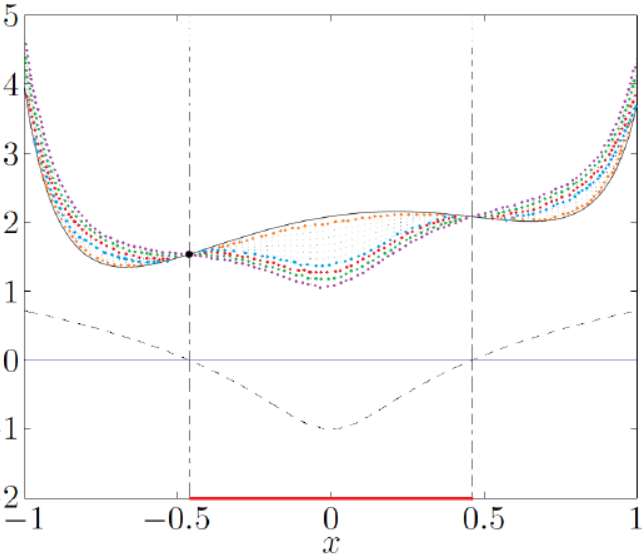
\includegraphics[height=5cm,width=6cm]{original_function_dual_problem.png}}
							%scale=0.6, height=4cm,width=4cm
							\qquad
							\subfigure[Dual function]{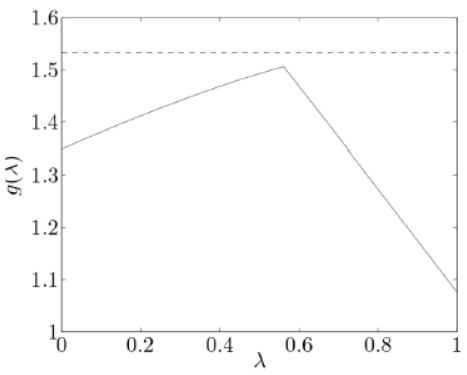
\includegraphics[height=5cm,width=6cm]{dual_function_dual_problem.png}}
							\renewcommand{\figurename}{Fig} % set picture title starting with Fig or 图
							\caption{ dual problem }
							\label{fig:9}
						\end{figure}
					
					
					SVM 里的 w,b 看做是 Lagrange 函数里的变量 x 
				\end{enumerate}
				
	\chapter{\quad SVM}
		\thispagestyle{fancy}
		\section{\quad linear separable support vector machine and hard margin maximization}
			\subsection{\quad question?} 
				\begin{figure}[H]
					\vspace{-0.2cm}  %调整图片与上文的垂直距离
					\setlength{\abovecaptionskip}{-0.2cm}   %调整图片标题与图距离
					%\setlength{\belowcaptionskip}{-1cm}   %调整图片标题与下文距离
					\centering
					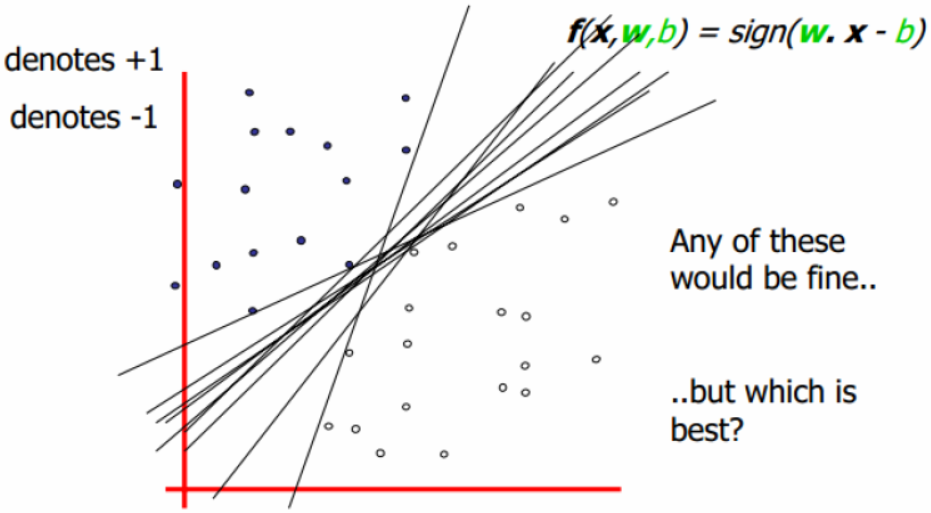
\includegraphics[scale=0.6]{linear_classifier.png}
					\renewcommand{\figurename}{Fig} % set picture title starting with Fig or 图
					\caption{linear classifier}
					\label{fig:10}
				\end{figure}
				
			\subsection{\quad input data} 
				\begin{enumerate}
					\item 假设给定有一个特征空间上的训练数据集 $T = \left\{ (x_1, y_1), (x_2, y_2), ..., (x_N, y_N) \right\}$
						其中, $x_i \in \boldsymbol{\text{R}}^n, y_i \in \left\{ +1, -1 \right\}, i=1,2,...,N $
						
					\item $x_i$ 为第 $i$ 个实例 (若 $n>1$, $x_i$ 为向量)
					
					\item $y_i$ 为 $x_i$ 的类标记
						\begin{enumerate}
							\item 当 $y = +1$ 时, 称 $x_i$ 为正例
							
							\item 当 $y = -1$ 时, 称 $x_i$ 为负例
						\end{enumerate}
					
					\item $(x_i, y_i)$ 称为样本点
				\end{enumerate}

			\subsection{\quad linear separable support vector machine}
				\begin{enumerate}
					\item 给定线性可分训练数据集, 通过 \textcolor{red}{间隔最大化} 得到的分离超平面为
						\begin{align}
							y(x) = w^T \phi(x) + b
						\end{align}
						相应的分类决策函数 
						\begin{align}
							f(x) = sign(w^T \phi(x) + b)
						\end{align}
						该决策函数称为线性可分支持向量机
						
					\item $\phi(x)$ 是某个确定的特征空间转换函数, 它的作用是将 $x$ 映射到 (更高的)维度
						\begin{enumerate}
							\item 最简单直接的 : $\phi(x) = x$
						\end{enumerate}
					
					\item 求解分离超平面问题可以等价为求解相应的 \textcolor{red}{凸二次规划问题}
				\end{enumerate}
	
			\subsection{\quad list symbol}
				\begin{enumerate}
					\item 分割平面: $y(x) = w^T \phi(x) + b$
		
					\item 训练集: $x_1, x_2, ..., x_n$
					
					\item 目标值: $y_1, y_2, ..., y_n, \quad y_i \in \left\{ -1, +1 \right\}$
					
					\item 新数据的分类: $sign(y(x))$
				\end{enumerate}
			
			\subsection{\quad derivation target function}
				\begin{enumerate}
					\item 根据题设 $y(x) = w^T \phi(x) + b$
					
					\item 有: 
						\begin{align}
							\left\{ 
								\begin{matrix}
									y(x_i) > 0 \Leftrightarrow y_i = +1\\
									y(x_i) < 0 \Leftrightarrow y_i = -1
								\end{matrix}
								\Rightarrow
								y_i \cdot y(x_i)>0
							\right.
						\end{align}
					
					\item functional margin and geometric margin
						\begin{figure}[H]
							\vspace{-0.2cm}  %调整图片与上文的垂直距离
							\setlength{\abovecaptionskip}{-0.2cm}   %调整图片标题与图距离
							%\setlength{\belowcaptionskip}{-1cm}   %调整图片标题与下文距离
							\centering
							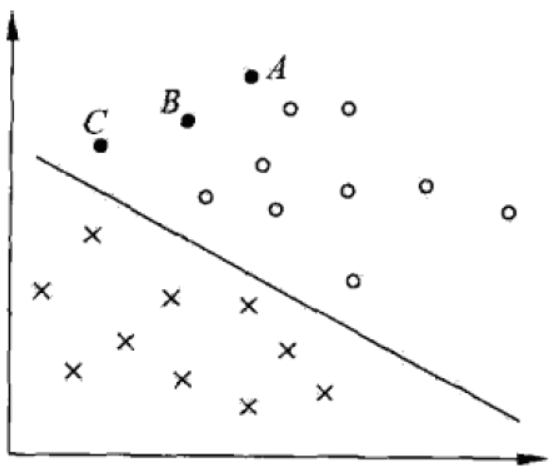
\includegraphics[scale=0.6]{functional_and_geometric_margin.png}
							\renewcommand{\figurename}{Fig} % set picture title starting with Fig or 图
							\caption{functional margin and geometric margin}
							\label{margin}
						\end{figure}
						\qquad 在图 \ref{margin} 中, 有 A,B,C 三个点, 表示3个实例, 均在分离超平面的正类侧, 预测它们的类, 点A距分离超平面较远, 若预测该点为正类, 就比较确信预测是正确的, 点C距分离超平面较劲, 若预测该点为正类就不么确信, 点B介于点A与C之间, 预测其为正类的确信度也在A与C之间
						\begin{itemize}
							\item \textcolor{red}{函数间隔}: 一般来说, 一个点距离分离超平面的远近可以表示分类预测的确信程度. 在超平面 $w^T \phi(x) + b = 0$ 确定的情况下, $|w^T \phi(x) + b|$ 能够相对地表示点 x 距离超平面的远近, 而 $w^T \phi(x) + b$ 的符号与类标记 y 的符号是否一致能够表示分类是否正确. 所以可用量 $y_i \cdot (w^T \cdot \phi(x_i) +_b$ 来表示分类的正确性及确信度.
						
							定义超平面 $(w, b)$ 关于样本点 $(x_i, y_i)$ 的函数间隔为
								\begin{align}
									\hat{\gamma}_i = y_i (w \cdot x_i + b)
 								\end{align}
						
							\item \textcolor{red}{几何间隔}: 函数间隔可以表示分类预测的正确性及确信度. 但是选择分离超平面时, 只有函数间隔还不够, 因为只要成比例的缩放 $w$ 和 $b$, 例如将它们改为 $2w$ 和 $2b$, 超平面并没有改变, 但函数间隔却成为原来的 2 倍, 这一事实启示我们, 可以对分离超平面的法向量 $\boldsymbol{w}$ 加某些约束, 如规范化, $\parallel w \parallel = 1$, 使得间隔是确定的. 这是函数间隔称为几何间隔.
							
							$w, b$ 等比例缩放, 则 $y_i*y$ 的值同样缩放, 从而:
							\begin{align}
								\gamma_i = \frac{y_i \cdot y(x_i)}{\parallel w \parallel} =
								\frac{y_i \cdot (w^T \cdot \phi(x_i) +_b)}{\parallel w \parallel}
							\end{align}
						\end{itemize}
					
					\item maximum margin to select separable hyperplane
						\begin{itemize}
							\item assume minimum functional margin and geometric margin 
							
								定义函数间隔平面 $(w, b)$ 关于 $T$ 中所有样本点 $(x_i, y_i)$ 的函数间隔之最小值, 即
								\begin{align}
								\hat{\gamma} = \min\limits_{i=1,...,N} \hat{\gamma_i}
								\end{align}
								
								定义几何间隔平面 $(w, b)$ 关于 $T$ 中所有样本点 $(x_i, y_i)$ 的几何间隔之最小值, 即
								\begin{align}
									\gamma = \min\limits_{i=1,...,N} \gamma_i
								\end{align}
							
							\item original target function
								\begin{align}
								&	\mathop{\arg\max}\limits_{w, b} \gamma
									=    \mathop{\arg\max}\limits_{w, b} 		\frac{\hat{\gamma}}{\parallel w \parallel}
									\Rightarrow\\
								&	\mathop{\arg\max}\limits_{w,b}
									 \left\{
										\frac{1}{\parallel w \parallel} \min\limits_{i}
										\left[ 
											y_i \cdot (w^T \cdot \phi(x_i) + b) 
										\right]
									\right\}\\
									&\text{s.t.} \quad \frac{y_i \cdot (w^T \cdot \phi(x_i) +_b)}{\parallel w \parallel} \geq \gamma
								\end{align}
								\begin{figure}[H]
									\vspace{-0.3cm}  %调整图片与上文的垂直距离
									\setlength{\abovecaptionskip}{-0.05cm}   %调整图片标题与图距离
									%\setlength{\belowcaptionskip}{-1cm}   %调整图片标题与下文距离
									\centering
									\subfigure[many optional hyperplane]{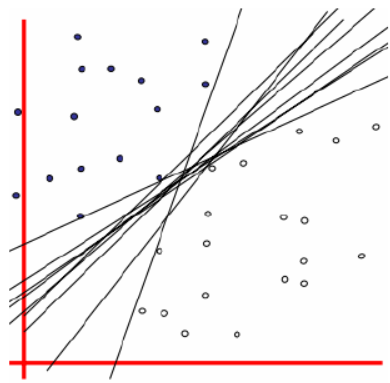
\includegraphics[height=5cm,width=6cm]{dataset.png}}
									%scale=0.6, height=4cm,width=4cm
									\qquad
									\subfigure[margin separable hyperplane]{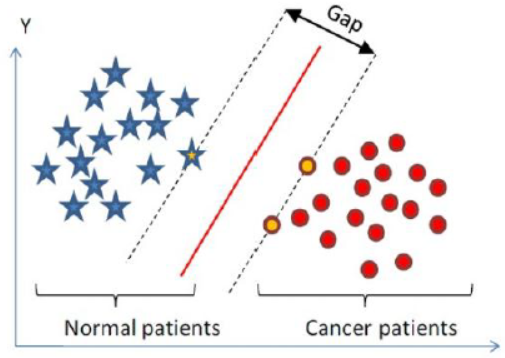
\includegraphics[height=5cm,width=6cm]{margin_separable_hyperplane.png}}
									\renewcommand{\figurename}{Fig} % set picture title starting with Fig or 图
									\caption{maximum margin}
									\label{fig:12}
								\end{figure}
							
							\item optimal problem
							
								\qquad 	\textcolor{red}{函数间隔 $\hat{\gamma} = y (w \cdot x + b)$ 不影响最优化问题的解.}  事实上, 假设将 $w$ 和 $b$ 按比例改变为 $\lambda w$ $\lambda b$, 这时函数间隔成为 $\lambda \hat{\gamma}$.
								
								\qquad 函数间隔的改变对上面最优化问题的不等式约束没有影响, 
								对目标函数的优化也没有影响. 即它产生一个等价的优化问题. 
								
								\qquad	取函数间隔最小值 $\hat{\gamma} = 1$. 将 $\hat{\gamma} = 1$ 代入上面的最优化问题, 注意到 最大化 $\frac{1}{\parallel w \parallel}$ 和 最小化 $\frac{1}{2} \parallel w \parallel ^2$ 是等价的. 则得到下面的 \textcolor{red}{线性可分支持向量机} 的最优化问题:
									\begin{align}
										\begin{split}
											&\min\limits_{w, b} \quad \frac{1}{2} \parallel w \parallel ^2
										\end{split} \label{basic_form_svm}\\
										&\text{s.t.} \quad y_i(w \cdot x_i + b) - 1 \geq 0, \quad i=1,2,...,N
									\end{align}
								\qquad 这是一个凸二次规划 (convex quadratic programming) 问题 :
								目标函数 $f(x)$ 是二次函数且约束函数 $g_i(w)$ 是仿射函数时, 约束最优化问题 (凸优化问题) 成为凸二次规划问题
						\end{itemize}
					
					\item dual algorithm
						\begin{enumerate}
							\item Lagrange multiplier method to build Lagrange function
								\begin{align}
									\begin{split}
										L(w, b, \alpha) = \frac{1}{2} \parallel w \parallel ^2 - \sum\limits_{i=1}^{n} \alpha_i (y_i (w^T \cdot \phi(x_i) + b) - 1)
									\end{split} \label{Lagrange_function}
								\end{align}
								among, $\alpha = (\alpha_1, \alpha_2, ..., \alpha_N)^T$ is Lagrange multiplier vector.
								
							\item 原问题是极小极大问题 $$\min\limits_{w,b} \max\limits_{\alpha} L(w, b, \alpha)$$
							原始问题的对偶问题, 是极大极小问题$$\max\limits_{\alpha} \min\limits_{w,b} L(w,b,\alpha)$$
							
							\item 得到对偶问题的解
								\begin{enumerate}[(1)]
									\item 求 $\min\limits_{w,b} L(w,b,\alpha)$\\
										将拉格朗日函数 $L(w,b,\alpha)$ 分别对 $w,b$ 求偏导数并令其等于0.
										\begin{align}
											\nabla_w L(w,b,\alpha) &= w - \sum_{i=1}^{N} \alpha_i y_i x_i= 0\\
											\nabla_b L(w,b,\alpha) &= \sum_{i=1}^{N} \alpha_i y_i = 0\\
											\text{得}\\
											\begin{split}
												w &= \sum_{i=1}^{N} \alpha_i x_i y_i
											\end{split} \label{derivation_w}\\
											\begin{split}
											\sum_{i=1}^{N} \alpha_i y_i &= 0
											\end{split}
											\label{derivation_y}
										\end{align}
										
									\item 将式 \ref{derivation_w} 代入Lagrange 函数 	\ref{Lagrange_function}, 并利用式 \ref{derivation_y}, 即得
										\begin{align}
											L(w,b,\alpha) &= \frac{1}{2} \parallel w \parallel ^2 - \sum_{i=1}^{n} \alpha_i (y_i(w^T \cdot \phi(x_i) + b) - 1)\\
											&= \frac{1}{2} w^T w - w^T \sum_{i=1}^{n} \alpha_i y_i \phi(x_i) - b\sum_{i=1}^{n} \alpha_i y_i + \sum_{i=1}^{n}\alpha_i\\
											&=\frac{1}{2}w^T \sum_{i=1}^{n}\alpha_i y_i \phi(x_i) - w^T \sum_{i=1}^{n}\alpha_i y_i \phi(x_i) - b\cdot 0 + \sum_{i-1}^{n}\alpha_i\\
											&= \sum_{i=1}^{n}\alpha_i - \frac{1}{2}\left( \sum_{i=1}^{n} \alpha_i y_i \phi(x_i) \right)^T \sum_{i=1}^{n}\alpha_i y_i \phi(x_i)\\
											&= \sum_{i=1}^{n}\alpha_i - \frac{1}{2}\sum_{i,j=1}^{n}\alpha_i \alpha_j y_i y_j \phi^T(x_i) \phi(x_j)				
										\end{align}
										即
										\begin{align}
											\min\limits_{w,b} L(w,b,\alpha) = -\frac{1}{2} \sum_{i=1}^{N}\sum_{i=1}^{N}\alpha_i \alpha_j y_i y_j \phi^T(x_i) \phi(x_j) + \sum_{i=1}^{N}\alpha_i
										\end{align}
										
									\item 求 $\min\limits_{w,b} L(w,b,\alpha)$ 对 $\alpha$ 的极大, 即是对偶问题
										\begin{align}
											&\max\limits_{\alpha} \quad \sum_{i=1}^{n} \alpha_i - \frac{1}{2} \sum_{i=1}^{n}\sum_{j=1}^{n} \alpha_i \alpha_j y_i y_j \left( \phi(x_i) \phi(x_j) \right)\\
											&\text{s.t.} \quad \sum_{i=1}^{n} \alpha_i y_i =0\\
											&\alpha_i \geq 0, \quad i=1,2,...,n
										\end{align}
										
									\item 整理目标函数: 添加负号
										\begin{align}
											&\min\limits_{\alpha} \quad \frac{1}{2} \sum_{i=1}^{n}\sum_{j=1}^{n} \alpha_i \alpha_j y_i y_j \left( \phi(x_i) \phi(x_j) \right) - \sum_{i=1}^{n} \alpha_i \\
											&\text{s.t.} \quad \sum_{i=1}^{n} \alpha_i y_i =0\\
											&\alpha_i \geq 0, \quad i=1,2,...,n
										\end{align}
								\end{enumerate}
						\end{enumerate}						
				\end{enumerate}
			
			\subsection{\quad Linear divisible support Vector Machine Learning algorithm}
				\begin{enumerate}
					\item 构造并求解约束最优化问题
						\begin{align}
							&\min\limits_{\alpha} \quad \frac{1}{2} \sum_{i=1}^{n}\sum_{j=1}^{n} \alpha_i \alpha_j y_i y_j \left( \phi(x_i) \phi(x_j) \right) - \sum_{i=1}^{n} \alpha_i \\
							&\text{s.t.} \quad \sum_{i=1}^{n} \alpha_i y_i =0\\
							&\alpha_i \geq 0, \quad i=1,2,...,n
						\end{align}
						
					\item 求得最优解 $\alpha^*$, $\alpha^* = (\alpha_1^*,\alpha_1^*,...,\alpha_1^* )^T$
					
					\item 计算
						\begin{align}
							w^* &= \sum_{i=1}^{N} \alpha_i^* y_i \phi(x_i)\\
							b^* &= y_i - \sum_{i=1}^{N} \alpha_i^* y_i (\phi(x_i) \cdot \phi(x_j))
						\end{align}
						
					\item 求得分离超平面
						\begin{align}
							w^* \phi(x) + b^* = 0
						\end{align}
						
					\item 分类决策函数
						\begin{align}
							f(x) = sign(w^* \phi(x) + b^*)
						\end{align}
						
					\item example
						\begin{enumerate}[]
							\item 						
								\begin{figure}[H]
									%\label{margin}
									\vspace{-0.2cm}  %调整图片与上文的垂直距离
									\setlength{\abovecaptionskip}{-0.2cm}   %调整图片标题与图距离
									%\setlength{\belowcaptionskip}{-1cm}   %调整图片标题与下文距离
									\centering
									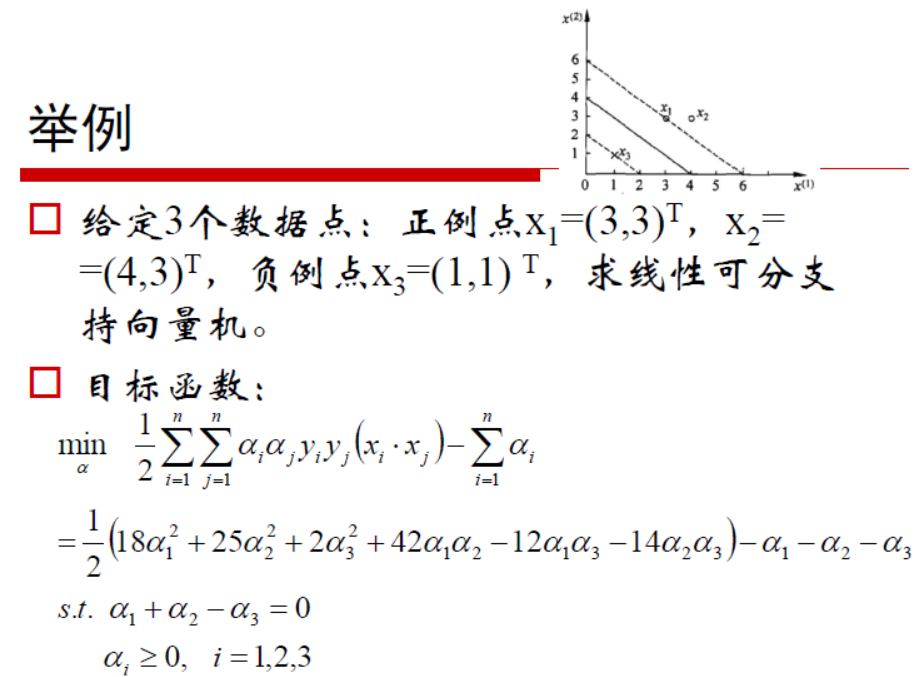
\includegraphics[scale=0.7]{separable_dataset_svm_example1.png}
									\renewcommand{\figurename}{Fig} % set picture title starting with Fig or 图
									%\caption{functional margin and geometric margin}
								\end{figure}
							
							\item 
								\begin{figure}[H]
									%\label{margin}
									\vspace{-0.2cm}  %调整图片与上文的垂直距离
									\setlength{\abovecaptionskip}{-0.2cm}   %调整图片标题与图距离
									%\setlength{\belowcaptionskip}{-1cm}   %调整图片标题与下文距离
									\centering
									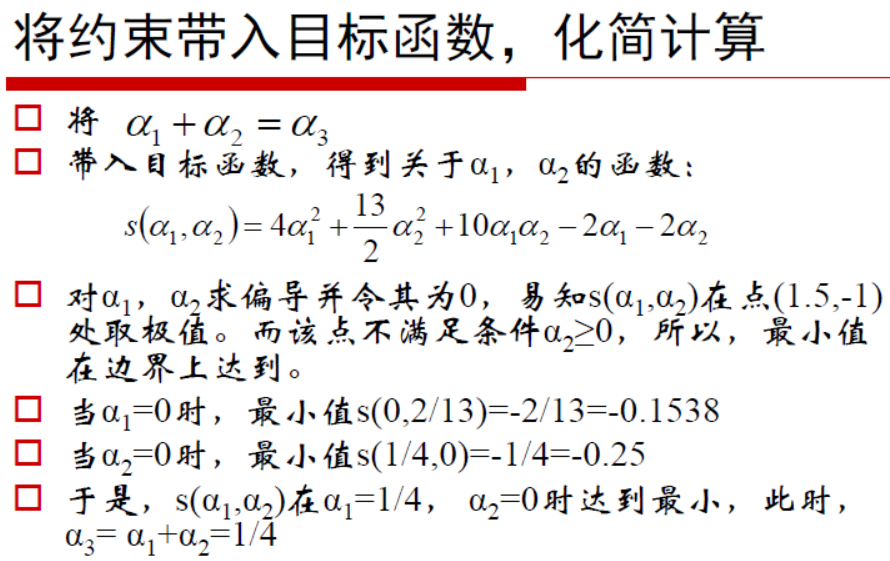
\includegraphics[scale=0.7]{separable_dataset_svm_example2.png}
									\renewcommand{\figurename}{Fig} % set picture title starting with Fig or 图
									%\caption{functional margin and geometric margin}
								\end{figure}
							
							\item 
								\begin{figure}[H]
									\label{fig:13}
									\vspace{-0.2cm}  %调整图片与上文的垂直距离
									\setlength{\abovecaptionskip}{-0.2cm}   %调整图片标题与图距离
									%\setlength{\belowcaptionskip}{-1cm}   %调整图片标题与下文距离
									\centering
									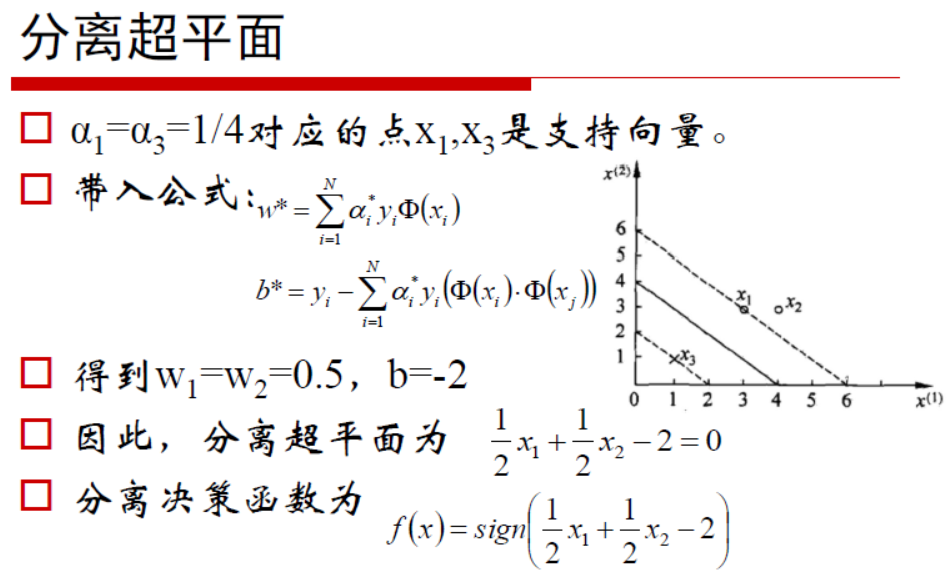
\includegraphics[scale=0.7]{separable_dataset_svm_example3.png}
									\renewcommand{\figurename}{Fig} % set picture title starting with Fig or 图
									\caption{the example of solve lagest margin separable hyperplane with svm method}
								\end{figure}							
						\end{enumerate}
				\end{enumerate}
			
		\section{\quad linear supprot vector machine and soft margin maximization}
			\subsection{\quad concept}
				\begin{enumerate}
					\item 不一定分类完全正确的超平面就是最好的
					
					\item 样本数据本身线性不可分
					
					\item picture
						\begin{figure}[H]
							\label{non_separable_dataset}
							\vspace{-0.2cm}  %调整图片与上文的垂直距离
							\setlength{\abovecaptionskip}{-0.2cm}   %调整图片标题与图距离
							%\setlength{\belowcaptionskip}{-1cm}   %调整图片标题与下文距离
							\centering
							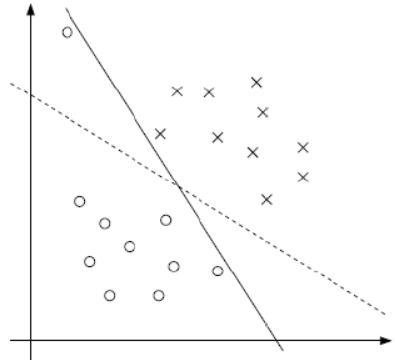
\includegraphics[scale=0.7]{non_separable_dataset.png}
							\renewcommand{\figurename}{Fig} % set picture title starting with Fig or 图
							\caption{non separable dataset}
						\end{figure}
				\end{enumerate}
			
			\subsection{\quad derivation target function}
				\begin{enumerate}
					\item 若数据线性不可分, 则增加松弛因子 $\xi \geq 0$, 使函数间隔加上松弛变量大于等于1. 这样, 约束条件变成
						\begin{align}
							y_i (w \cdot x_i + b) \geq 1 - \xi
						\end{align}
						
					\item target function with adding slack variable $\xi$:
						\begin{align}
							\min\limits_{w,b} \frac{1}{2} \parallel w \parallel ^2 + C \sum_{i=1}^{N} \xi_i
						\end{align}
						
					\item this moment, the target function of linear svm
						\begin{align}
							&\min\limits_{w,b,\xi} \quad \frac{1}{2} \parallel w \parallel ^2 + C \sum_{i=1}^{N} \xi_i\\
							&\text{s.t.} \quad y_i(w \cdot x_i + b) \geq 1 - \xi_i, \quad i=1,2,...,n\\
							&\xi_i \geq 0, \quad i=1,2,...,n
						\end{align}
				\end{enumerate}
			
			\subsection{\quad dual property}
				\begin{enumerate}
					\item Lagrange 函数
						\begin{align}
							\begin{split}
								L(w,b,\xi,\alpha,\mu) = \frac{1}{2} \parallel w \parallel^2 + C\sum_{i=1}^{n}\xi_i - \sum_{i=1}^{n}\alpha_i(y_i(w \cdot x_i + b) - 1 + \xi_i) - \sum_{i=1}^{n}\mu_i \xi_i
							\end{split} \label{Lagrange_function_linear_svm}
						\end{align}
						
					\item 对 $w,b,\xi$ 求偏导
						\begin{align}
							\begin{split}
								&\frac{\partial L}{\partial w} = 0 \Rightarrow w = \sum_{i=1}^{n} \alpha_i y_i \phi(x_n) 
							\end{split} \label{partial_w_linear_svm}\\
							\begin{split}
								&\frac{\partial L}{\partial b} = 0 \Rightarrow 0 = \sum_{i=1}^{n} \alpha_i y_i 
							\end{split} \label{partial_b_linear_svm}\\
							\begin{split}
								&\frac{\partial L}{\partial \xi} = 0 \Rightarrow C - \alpha_i - \mu_i = 0 
							\end{split} \label{partial_xi_linear_svm}
						\end{align}
						
					\item 将式 \ref{partial_w_linear_svm} 、式 \ref{partial_b_linear_svm} 、式 \ref{partial_xi_linear_svm} 代入式 \ref{Lagrange_function_linear_svm} 中, 得到
						\begin{align}
							\begin{split}
								\min\limits{w,b,\xi} L(w,b,\xi,\alpha,\mu) = - \frac{1}{2}\sum_{i=1}^{n}\sum_{j=1}^{n} \alpha_i\alpha_j y_i y_j (x_i \cdot x_j) + \sum_{i=1}^{n}\alpha_i
							\end{split} \label{dual_Lagrange_function_linear_svm}
						\end{align}
						
					\item 对上式 \ref{dual_Lagrange_function_linear_svm} 求关于 $\alpha$ 的极大, 得到
						\begin{align}
							\begin{split}
								\max\limits_{\alpha} \quad &- \frac{1}{2}\sum_{i=1}^{n}\sum_{j=1}^{n} \alpha_i\alpha_j y_i y_j (x_i \cdot x_j) + \sum_{i=1}^{n}\alpha_i 
							\end{split} \label{maximum_alpha}
							\\
							\begin{split}
								\text{s.t.} \quad &\sum_{i=1}^{n} \alpha_i y_i = 0 \label{alpha_equal_maximum_alpha_restrict}
							\end{split}
							 \\
							\begin{split}
								&C -\alpha_i -\mu_i = 0 \label{alpha_mu_equal_maximum_alpha_restrict}
							\end{split}
							 \\
							\begin{split}
								&\alpha_i \geq 0 \label{domain_alpha}
							\end{split}
							\\
							\begin{split}
								&\mu_i \geq 0, \quad i=1,2,..,n \label{domain_mu}
							\end{split}	
						\end{align}
						
					\item 将对偶问题 \ref{maximum_alpha} $\sim$ \ref{domain_mu} 进行变换: 利用等式约束 \ref{alpha_mu_equal_maximum_alpha_restrict} 消去 $\mu_i$, 从而只留下变量 $\alpha_i$, 并将约束 \ref{alpha_mu_equal_maximum_alpha_restrict} $\sim$ \ref{domain_mu} 写成
						\begin{align}
							0 \leq \alpha_i \leq C
						\end{align}
						
					\item 整理, 得到对偶问题:
						\begin{align}
							\min\limits_{\alpha} \quad & \frac{1}{2}\sum_{i=1}^{n}\sum_{j=1}^{n} \alpha_i\alpha_j y_i y_j (x_i \cdot x_j) - \sum_{i=1}^{n}\alpha_i \\
							\text{s.t.} \quad &\sum_{i=1}^{n} \alpha_i y_i = 0\\
							&0 \leq \alpha_i \leq C, \quad i=1,2,...,n
						\end{align}
				\end{enumerate}
			
			\subsection{\quad Linear support vector machine learning algorithm}
				\begin{enumerate}
					\item 构造并求解约束最优化问题
						\begin{align}
							\begin{split}
								\min\limits_{\alpha} \quad & \frac{1}{2}\sum_{i=1}^{n}\sum_{j=1}^{n} \alpha_i\alpha_j y_i y_j (x_i \cdot x_j) - \sum_{i=1}^{n}\alpha_i
							\end{split} \label{target_function_linear_svm} \\
							\begin{split}
								\text{s.t.} \quad &\sum_{i=1}^{n} \alpha_i y_i = 0
							\end{split} \label{equal_restrict_linear_svm} \\
							\begin{split}
								&0 \leq \alpha_i \leq C, \quad i=1,2,...,n
							\end{split} \label{alpha_restrict_linear_svm}
						\end{align}
						
					\item 求得最优解 $\alpha^*$, $\alpha^* = (\alpha_1^*,\alpha_2^*,...,\alpha_n^*)^T$
					
					\item 计算
						\begin{align}
							w^* = \sum_{i=1}^{n} \alpha_i^* y_i x_i
						\end{align}
						计算 b 的值有两种方式:
						\begin{itemize}
							\item 选择 $\alpha^*$ 的一个分量 $\alpha_j^*$ 适合条件 $0 < \alpha_j^* < C$, 计算
								\begin{align}
									b^* = y_j - \sum_{i=1}^{n}y_i \alpha_i^*(x_i \cdot x_j)
								\end{align}
							
							\item 实践中往往取支持向量的所有值取平均, 作为 $b^*$
								\begin{align}
									b^* = \frac{\max\limits_{i: y_i=-1} w^* \cdot x_i + \min\limits_{i: y_i=1} w^* \cdot x_i}{2}
								\end{align}
						\end{itemize}
						
					\item 求得分离超平面
						\begin{align}
							w^* x + b^* = 0
						\end{align}
						
					\item 分类决策函数
						\begin{align}
							f(x) = sign(w^* x + b^*)
						\end{align}
				\end{enumerate}
			
			\subsection{\quad KKT of soft margin}
				\begin{align}
					\nabla_w L(w^*, b^*, \xi^*, \alpha^*, \mu^*) &= w^* - \sum_{i=1}^{N} \alpha_i^* y_i x_i = 0 \\
					\nabla_b L(w^*, b^*, \xi^*, \alpha^*, \mu^*) &= -\sum_{i=1}^{N} \alpha_i^* y_i = 0 \\
					\nabla_\xi L(w^*, b^*, \xi^*, \alpha^*, \mu^*) &= C - \alpha^* - \mu^* = 0 \\
					\begin{split}
						\alpha_i^* (y_i(w^* \cdot x_i + b^*)& - 1 + \xi_i^*) = 0
					\end{split} \label{alpha_euqal_restrict_kkt_soft_margin}
					\\
					\begin{split}
						\mu_i^* \xi_i^* &= 0
					\end{split} \label{xi_equal_restrict_kkt_soft_margin}
					\\
					\begin{split}
						y_i(w^* x_i + b^*) &- 1 + \xi^* \geq = 0
					\end{split} \label{not_equal_restrict_kkt_soft_margin}
					\\
					\xi_i^* &\geq 0\\
					\alpha_i^* &\geq 0\\
					\mu_i^* &\geq 0, \quad i=1,2,...,N
				\end{align}
			
			\subsection{\quad support vector}
				\begin{enumerate}
					\item 在线性不可分的情况下, 将对偶问题 \ref{target_function_linear_svm} $\sim$ \ref{alpha_restrict_linear_svm} 的解 $\alpha^* = (\alpha_1^*,\alpha_2^*,...,\alpha_n^*)^T$ 中对应于 $\alpha_i^* > 0$ 的样本点 $(x_i, y_i)$ 的实例 $x_i$ 称为支持向量(软间隔的支持向量). 
						\begin{figure}[H]
							\label{support_vector_soft_margin_linear_svm}
							\vspace{-0.2cm}  %调整图片与上文的垂直距离
							\setlength{\abovecaptionskip}{-0.2cm}   %调整图片标题与图距离
							%\setlength{\belowcaptionskip}{-1cm}   %调整图片标题与下文距离
							\centering
							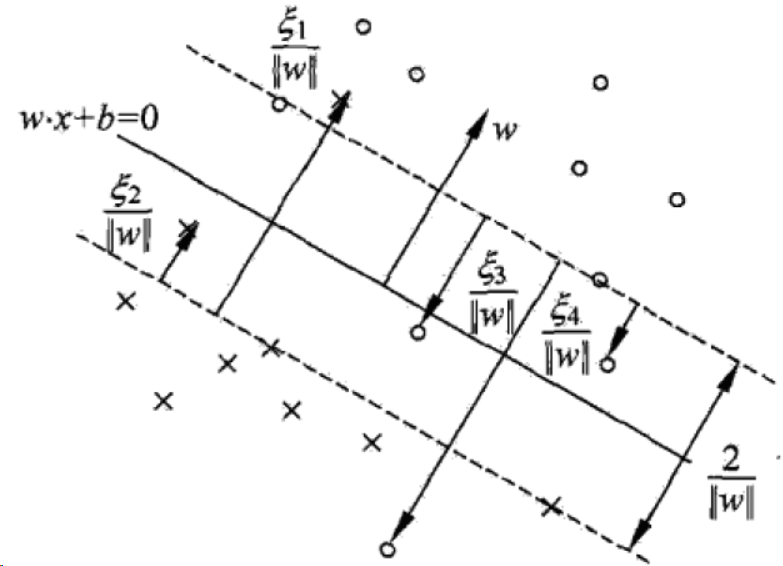
\includegraphics[scale=0.6]{support_vector_soft_margin_linear_svm.png}
							\renewcommand{\figurename}{Fig} % set picture title starting with Fig or 图
							\caption{support vector soft margin linear svm}
						\end{figure}
						这时的支持向量要比线性可分时的情况复杂一些. 图中, 分离超平面由实线表示, 间隔边界由虚线表示, 正例点由 “。” 表示, 负例点由 "$\times$"表示. 图中还标出了实例 $x_i$ 到间隔边界的距离 $\frac{\xi}{\parallel w \parallel}$
						
						\textcolor{red}{软间隔的支持向量 $x_i$  或者在间隔边界上, 或者在间隔边界与分离超平面之间, 或者在分离超平面误分一侧.}
						
						KKT条件中式 \ref{alpha_euqal_restrict_kkt_soft_margin}、 \ref{xi_equal_restrict_kkt_soft_margin}、 \ref{not_equal_restrict_kkt_soft_margin} 得出目标函数中 $\alpha_i$ 取值的意义:
						\begin{enumerate}
							\item 在两条间隔线外面的点, 对应前面的系数 $\alpha_i$ 为 0, 
								\begin{align}
									\xi = 0, y_i(w^* x + b) -1 + \xi > 0 \Leftrightarrow  \alpha_i = 0 
								\end{align}
								
							\item 在两条间隔线里面的对应 $\alpha_i$ 为 C,
								\begin{itemize}
									\item 支持向量落在间隔边界和分离超平面之间
										\begin{align}
											&0 < \xi < 1 \Leftrightarrow \notag \\
											 &\mu =0, \alpha_i = C, y_i(w^* x + b) -1 + \xi = 0, 0 < y_i(w^* x + b) < 1 
										\end{align}
										
									\item 支持向量落在分离超平面上
										\begin{align}
											&\xi = 1 \Leftrightarrow \notag \\
											&\mu =0, \alpha_i = C, y_i(w^* x + b) -1 + \xi = 0,  y_i(w^* x + b) = 0  
										\end{align}
										
									\item 支持向量位于分离超平面误分一侧
										\begin{align}
											&\xi > 1 \Leftrightarrow \notag \\
											&\mu =0, \alpha_i = C, y_i(w^* x + b) -1 + \xi = 0, y_i(w^* x + b) < 0  
										\end{align}
								\end{itemize}
								
							\item 在两条间隔线上的对应的系数 $\alpha_i$ 在 0 和 C 之间
								\begin{align}
									&\xi = 0, y_i(w^* x + b) -1 = 0 \Leftrightarrow \notag \\
									&0 \leq \mu \leq C, 0 \leq \alpha \leq C, y_i(w^* x + b) -1 + \xi = 0
								\end{align}
						\end{enumerate}							
				\end{enumerate}
			
			\subsection{\quad loss function}
				\begin{enumerate}
					\item $l_{0/1}$ loss function
				
						在软间隔允许某些样本不满足约束 
							\begin{align}
								y_i(w^T x_i + b) \geq 1 \label{restrict_0_1_loss_function}
							\end{align}\
						在最大化间隔时, 不满足的样本应尽可能少, 则优化目标为
							\begin{align}
								\begin{split}
									\min\limits_{w,b} \frac{1}{2} \parallel w \parallel ^2 + C\sum_{i=1}^{m} l_{0/1} (y_i(w^T x_i + b) -1)
								\end{split} \label{0_1_loss_function}
							\end{align}
						其中, $C>0$ 是一个常数, $l_{0/1}$ 是"0/1损失函数"
							\begin{align}
								l_{0/1}(z) = \left\{
								\begin{matrix}
									&1, \quad &\text{if} \ z<0;\\
									&0, \quad &\text{otherwise}
								\end{matrix}
								\right.
							\end{align}
						
						显然, 当C为无穷大时, 式 \ref{0_1_loss_function} 迫使所有样本满足约束 \ref{restrict_0_1_loss_function}, 于是式 \ref{0_1_loss_function} 等价于式 \ref{basic_form_svm}; 当 C 取有限制时, 式 \ref{0_1_loss_function} 允许一些样本不满足约束
						
						
					\item surrogate loss 替代损失
						
						因为 $l_{0/1}$ 非凸、非连续, 数学性质不好, 使得式 \ref{0_1_loss_function} 不易直接求解.
						
						于是, 通常用其他一些函数来代替 $l_{0/1}$ , 称为 "替代损失"
						
						替代损失函数一般具有较好的数学性质, 如它们通常是凸的连续函数且是 $l_{0/1}$ 的上届.
						
					\item $l_{0/1}$ 损失函数、 hinge 损失函数、 指数损失函数、 对率损失函数
					 	\begin{figure}[H]
						 	%\label{Fig:three_surrogate_loss_function}
						 	\vspace{-0.2cm}  %调整图片与上文的垂直距离
						 	\setlength{\abovecaptionskip}{-0.2cm}   %调整图片标题与图距离
						 	%\setlength{\belowcaptionskip}{-1cm}   %调整图片标题与下文距离
						 	\centering
						 	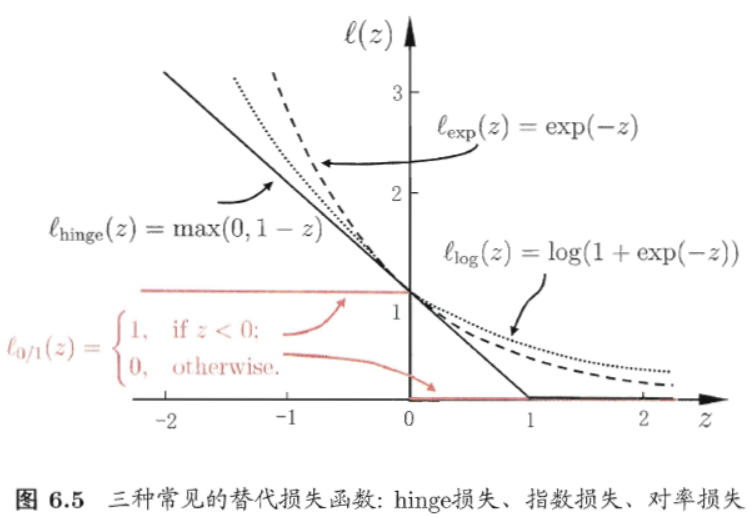
\includegraphics[scale=0.8]{three_surrogate_loss_function.png}
						 	\renewcommand{\figurename}{Fig} % set picture title starting with Fig or 图
						 	\caption{three surrogate loss function}
						 	\label{Fig:three_surrogate_loss_function}
					 	\end{figure}
					
					\item hinge 损失:
							\begin{align}
								l_{hinge}(z) = \max(0, 1-z)
							\end{align}
						  指数损失函数:
						  	\begin{align}
						  		l_{exp}(z) = \text{exp}(-z)
						  	\end{align}
						  对率损失:
						  	\begin{align}
						  		l_{log}(z) = \log(1 + \text{exp}(-1))
						  	\end{align}
						  	
					\item 若采用 hinge 损失, 则式 \ref{0_1_loss_function} 变成
						\begin{align}
							\min\limits_{w,b} \frac{1}{2} \parallel w \parallel ^2 + C\sum_{i=1}^{m} \max(0, 1 - y_i(w^T x_i + b)) \label{hinge_loss_function}
						\end{align}
					
					\item 引入松弛变量 $\xi_i \geq 0$, 可将式 \ref{hinge_loss_function} 重写为
						\begin{align}
							\min_{w,b,\xi_i} \frac{1}{2} \parallel w \parallel ^2 + C\sum_{i=1}^{m}\xi_i 
						\end{align}
						
					\item 图 \ref{Fig:three_surrogate_loss_function} 中, 横轴是函数间隔 $y(w \cdot x + b)$,纵轴是损失.
					
						0-1 损失函数是二分类问题的真正的损失函数, 而合页损失函数是 0-1 损失函数的上界. 
						\begin{figure}[H]	
							\vspace{-0.2cm}  %调整图片与上文的垂直距离
							\setlength{\abovecaptionskip}{-0.2cm}   %调整图片标题与图距离
							%\setlength{\belowcaptionskip}{-1cm}   %调整图片标题与下文距离
							\centering
							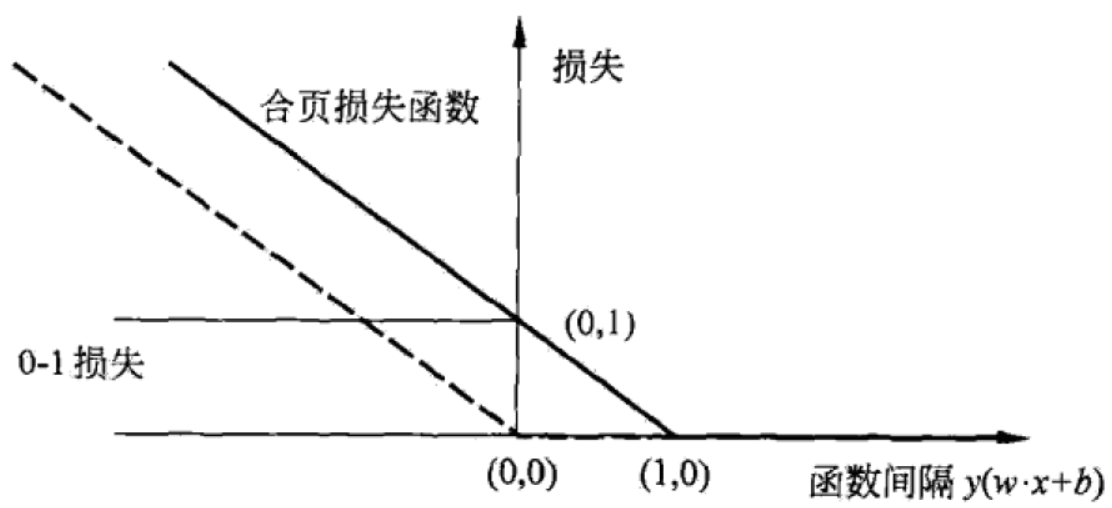
\includegraphics[scale=0.4]{hinge_loss_function.png}
							\renewcommand{\figurename}{Fig} % set picture title starting with Fig or 图
							\caption{hinge loss function}
							\label{Fig:hinge_loss_function}
						\end{figure}
						图 \ref{Fig:hinge_loss_function} 中虚线显示的是感知机的损失函数 $[-y_i (w \cdot x_i + b)]_+$. 
						
						当样本点 $(x_i, y_i)$ 点被分类正确时, 损失是0, 否则损失是 $-y_i(w \cdot x_i + b)$.
						
						相比之下, 合页损失函数不仅要分类正确, 而且确信度足够高时损失才是 0. 也就是说, 合页损失函数对学习有更高的要求.
				\end{enumerate}
				
		\section{\quad kernel function}
			如果样本线性不可分, 通过 $\phi : X \rightarrow F$ 函数映射将输入样本映射到另外一个高维空间并使其线性可分.
			
			将内积 $<x_i, x_j>$ 变成 $<\phi(x_i), \phi(x_j)>$
			
			求解 $<\phi(x_i), \phi(x_j)>$ 有两种方法:
				\begin{enumerate}
					\item 先找到这种映射 $\phi(x)$, 然后将输入空间中的样本映射到新的空间中, 最后在新空间中取求内积 $<\phi(x_i), \phi(x_j)>$
					
					\item 核技巧: 不显示的定义映射函数 $\phi(x)$, 值定义核函数 $K(x_i, x_j)$
				\end{enumerate}
			
			\subsection{\quad define directily reflect function}
				以多项式 $x_1 + x_2 + x_1^2 + x_2^2 + c = 0$ 为例
				
				将其进行变换, $c_1 = x_1, c_2 = x_2, c_3 = x_1^2, c_4 = x_2^2$, 得到:
				$c_1 + c_2 + c_3 + c_4 = 0$, 也就是说通过把输入空间从二维向四维映射后, 样本有线性不可分变成了线性可分, 但是这种转化带来的直接问他是维度变高了, 这意味着, 首先可能导致后续计算变复杂, 其次可能出现维度灾难.
				
				对于学习器而言就是: 特征空间维数可能最终无法计算, 而它的泛化能力 (学习器对训练样本以外数据的适应性) 会随着维度的增大而大大降低, 这也违反了 "奥坎姆剃刀", 最终可能使内积 $<\phi(x_i), \phi(x_j)>$ 无法求出, 于是也就失去这种转化的优势了
				
				
			\subsection{\quad kernel function}
				\begin{enumerate}
					\item concept
						
						definition one: 核是一个函数 K, 对于所有的 $x_1, x_2 \in X$ 满足, $K<x_1, x_2> = <\phi(x_1), \phi(x_2)>$, 这里的 $\phi$ 为从 X 到内积特征空间 F 的映射
					
					\item picture
						\begin{figure}[H]	
							\vspace{-0.2cm}  %调整图片与上文的垂直距离
							\setlength{\abovecaptionskip}{-0.2cm}   %调整图片标题与图距离
							%\setlength{\belowcaptionskip}{-1cm}   %调整图片标题与下文距离
							\centering
							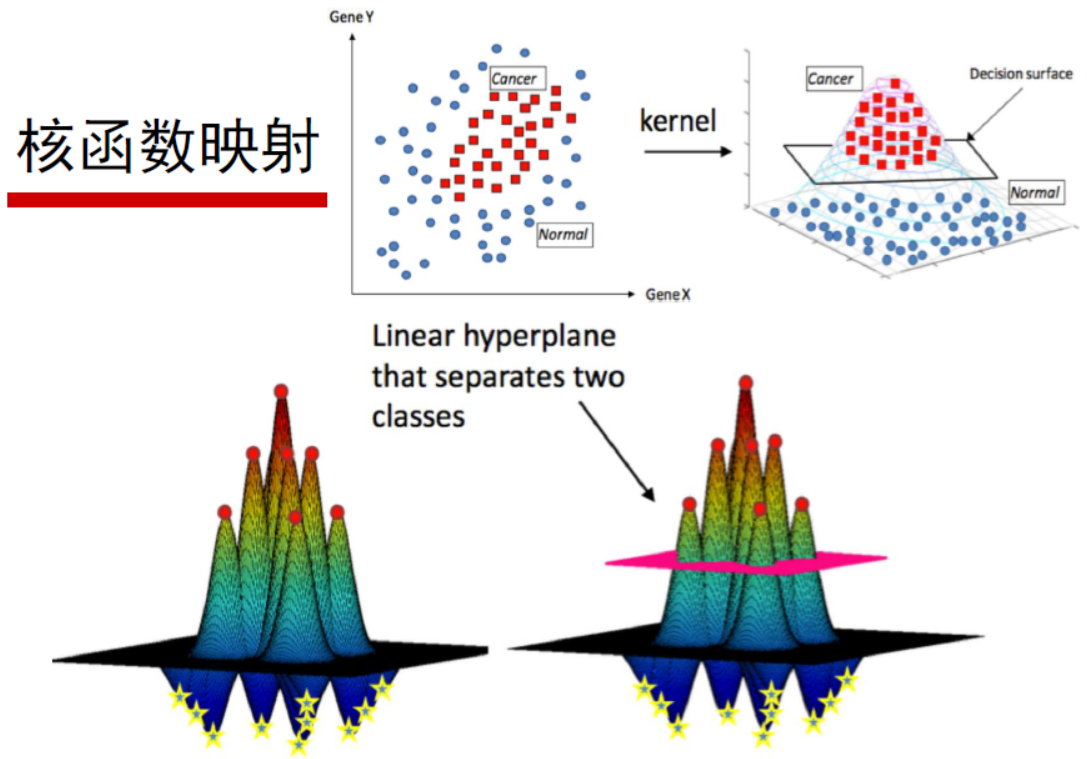
\includegraphics[scale=0.6]{reflect_kernel_function.png}
							\renewcommand{\figurename}{Fig} % set picture title starting with Fig or 图
							\caption{reflect kernel function}
							\label{Fig:reflect_kernel_function}
						\end{figure}
					
					\item condition
					
						$K(x, y)$ 什么时候才是核函数呢?
						
						假设有输入有输入空间 $X = x_1, x_2, ..., x_n$ 且 $K(x, y)$ 为对称函数, 那么对于所有样本得到下面矩阵: $k = K(x_i, x_j) (i,j = 0,...,n)$, 显然, 这个是对称矩阵, 那么对于对称矩阵一定存在一个正交矩阵, 使得 $P^T k P = \Lambda$, 这里 $\Lambda$ 是包含 $k$ 的特征值 $\lambda_i$ 的对角矩阵, 特征值 $\lambda_i$ 对应的特征向量为 $\nu_{i} = (\nu_{i1}, \nu_{i2}, ..., \nu_{in})^T$, 其中 n 为样本数, 对输入空间做如下映射 $\phi$
							\begin{align}
								&\phi (x_i) \Rightarrow (\sqrt{\lambda_1} \nu_{1i}, \sqrt{\lambda_2} \nu_2i, ..., \sqrt{\lambda_n} \nu_ni)^T \in R^n (i=1,2,...,n)\\
								&\phi(x) = \left(\phi(x_1), \phi(x_2), ..., \phi(x_n)\right)\\
								&K(x_i,x_j) = \phi(x_i)^T \phi(x_j)
							\end{align}
							
						于是有 $<\phi(x_i), \phi(x_j)> = \sum_{t=1}^{n} \lambda_t \nu_{ti} \nu_{tj} = (V \Lambda V^T)_{i,j} = k_{i,j} = K(x_i, x_j)$ (其中 V 为特征向量组成的矩阵, $\Lambda$ 为相应特征值组成的三角矩阵), 也就是说 K 是对应于映射的核函数.
						
					\item example
						
						有 $k = \left[ \begin{matrix}
						4 \ 0 \ 0 \\ 0 \ 3 \ 1 \\ 0 \ 1 \ 3
						\end{matrix} \right]$, 由
						$|k - \lambda E| = 0$ 解得特征值: $\lambda_1 = \lambda_2 = 4$, $\lambda_3 = 2$, 对 2 重特征根 4 求  $(A-4E)x = 0$ 的基础解系、正交化、单位化后得到特征向量: $\nu_1 = (1,0,0)^T$ 和 $\nu_2 = (0, \frac{1}{\sqrt{2}}, \frac{1}{\sqrt{2}})^T$, 对 $\lambda_3$ 的特征向量单位化后得到 $\nu_3 = (0, -\frac{1}{\sqrt{2}}, \frac{1}{\sqrt{2}})^T$, 于是有
							$V = (\nu_1, \nu_2, \nu_3) = \begin{vmatrix}
								1 & 0 & 0\\
								0 & \frac{1}{\sqrt{2}} & -\frac{1}{\sqrt{2}}\\
								0 & \frac{1}{\sqrt{2}} & \frac{1}{\sqrt{2}}
							\end{vmatrix}$
						满足$V^{-1} k V = \Lambda = \begin{bmatrix}
								4 & 0 & 0\\
								0 & 4 & 0\\
								0 & 0 & 2
						\end{bmatrix}$, 对所有输入样本做映射得:
						\begin{align}
							&\phi(x_1) = (\sqrt{4}\times 1, \sqrt{4} \times 0, \sqrt{2} \times 0)^T = (2,0,0)^T;\\
							&\phi(x_2) = (\sqrt{4}\times 0, \sqrt{4} \times \frac{1}{\sqrt{2}}, \sqrt{2} \times -\frac{1}{\sqrt{2}})^T = (0,\sqrt{2},-1)^T;\\
							&\phi(x_3) = (\sqrt{4}\times 0, \sqrt{4} \times \frac{1}{\sqrt{2}}, \sqrt{2} \times \frac{1}{\sqrt{2}})^T = (0,\sqrt{2},1)^T
						\end{align}
						随便选两个做内积, 如 $<\phi(x_2), \phi(x_3)> = 0 \times 0 + \sqrt{2} \times \sqrt{2} + (-1)\times 1 = 1 = k(x_2, x_3)$
						
						由此可见: $K(x,y)$ 就是对应于特征映射 $\phi(x)$ 的核函数 
						
					\item conclusion
						\begin{itemize}
							\item 定理1: 存在有限输入空间 X, K(x,y) 为 X 上的对称函数, 那么 K(x,y) 是核函数的冲要条件是矩阵 $k = (K(x_i, x_j)) (i,j=0,...,n)$ 半正定, 此时相当于对输入空间想特征空间进行了 \textcolor{red}{隐式} 的 $\phi(x)$ 映射. 对于上面的映射 $\phi(x)$, 令 $\phi_i(x_j) = \sqrt{\lambda_i} \nu_{ij}$,于是 $\phi(x) = (\phi_1(x), \phi_2(x), ..., \phi_n(x))$
							
							\item 令 $\chi$ 为输入空间, $\kappa(\cdot,\cdot)$ 是定义在 $\chi \times \chi$ 上的对称函数, 则 $\kappa$ 是核函数当且仅当对于任意数据 $D = \left\{ x_1, x_2, ..., x_n \right\}$, kernel matrix K 总是半正定的
							\begin{align}
								\boldsymbol{K} = 
									\begin{bmatrix}
										&\kappa(x_1,x_1) &\cdots &\kappa(x_1,x_j) &\cdots &\kappa(x_1,x_m)\\
										&\vdots & \ddots &\vdots &\ddots &\vdots\\
										&\kappa(x_i,x_1) &\cdots &\kappa(x_i,x_j) &\cdots &\kappa(x_i,x_m)\\
										&\vdots &\ddots &\vdots &\ddots &\vdots\\
										&\kappa(x_m,x_1) &\cdots &\kappa(x_m,x_j) &\cdots &\kappa(x_m,x_m)
									\end{bmatrix}
							\end{align} 
							事实证明, 只要一个对称函数所对应的核矩阵半正定, 它就能作为核函数使用. 事实上, 一个半正定核矩阵, 总能找到一个与之对应的映射 $\phi$, 换言之, 任何一个核函数都隐式得定义了一个称为 “再生核希尔伯特空间” 的特征空间
						\end{itemize}
					
					\item common kernel function
						\begin{table}
							\centering
							\vspace{-1cm}
							%\scriptsize
							%\renewcommand{\tablename}{\xiaosihao\HEI table}
							\setlength{\belowcaptionskip}{0.2cm}   %调整图片标题与图距离
							\renewcommand{\tablename}{Tab}
							\caption{common kernel function}						
							\begin{tabular}{l l l}
								\hline
								名称 &表达式 &参数\\
								\hline
								线性核 &$\kappa(x_i,x_j) = x_i^T x_j$ &\\
								多项式核 &$\kappa(x_i,x_j) = (x_i^T x_j)^d$ &$d \geq 1$为多项式的次数\\
								高斯核 &$\kappa(x_i,x_j) = \text{exp}(-\frac{\parallel x_i - x_j \parallel^2}{2\sigma^2})$ &$\sigma>0$ 为高斯核的带宽 (width)\\ 
								拉普拉斯核 &$\kappa(x_i,x_j) = \text{exp}(-\frac{\parallel x_i - x_j \parallel}{\sigma})$ &$\sigma>0$\\
								Sigmoid核 &$\kappa(x_i,x_j) = \tanh(\beta x_i^T x_j + \theta)$ &$\tanh \text{为双曲正切函数}, \beta>0, \theta<0$\\
								\hline
							\end{tabular}
						\end{table}
					
					\item Gussian kernel function
					
						在实际应用中, 往往依赖先验领域知识 / 交叉验证等方案才能选择有效的核函数. 
						
						没有更多先验信息, 则使用高斯核函数
						\begin{enumerate}[]
							\item 						
							\begin{figure}[H]
								%\label{concept_gussian_kernel_function}
								\vspace{-0.2cm}  %调整图片与上文的垂直距离
								\setlength{\abovecaptionskip}{-0.2cm}   %调整图片标题与图距离
								%\setlength{\belowcaptionskip}{-1cm}   %调整图片标题与下文距离
								\centering
								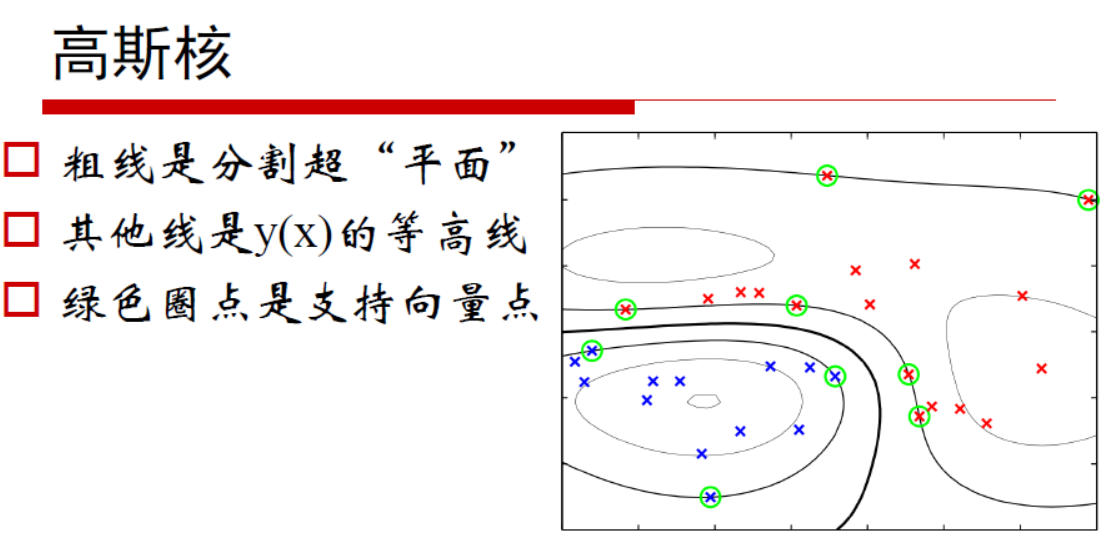
\includegraphics[height=7cm,width=14cm]{concept_gussian_kernel_function.png}
								\renewcommand{\figurename}{Fig} % set picture title starting with Fig or 图
								%\caption{concept gussian kernel function}
							\end{figure}
							
							\item 
							\begin{figure}[H]
								\centering
								%\label{theory_gussian_kernel_function}
								\vspace{-0.2cm}  %调整图片与上文的垂直距离
								\setlength{\abovecaptionskip}{-0.2cm}   %调整图片标题与图距离
								%\setlength{\belowcaptionskip}{-1cm}   %调整图片标题与下文距离
								
								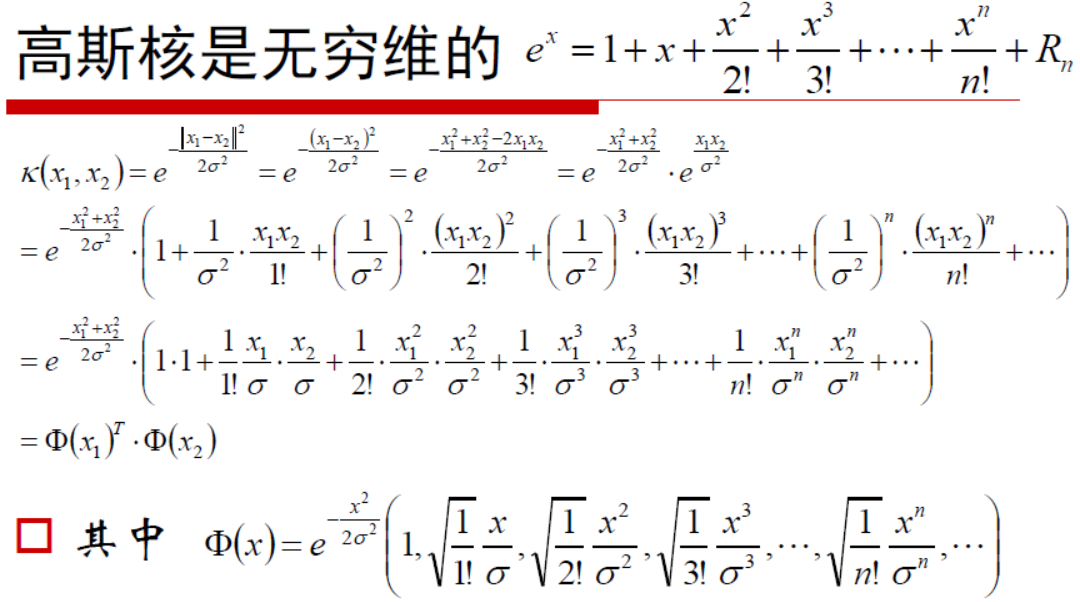
\includegraphics[height=9cm,width=14.5cm]{theory_gussian_kernel_function.png}
								\renewcommand{\figurename}{Fig} % set picture title starting with Fig or 图
								%\caption{theory gussian kernel function}
							\end{figure}
							
							\item 
							\begin{figure}[H]
								\label{result_gussian_kernel_function}
								\vspace{-0.2cm}  %调整图片与上文的垂直距离
								\setlength{\abovecaptionskip}{-0.2cm}   %调整图片标题与图距离
								%\setlength{\belowcaptionskip}{-1cm}   %调整图片标题与下文距离
								\centering
								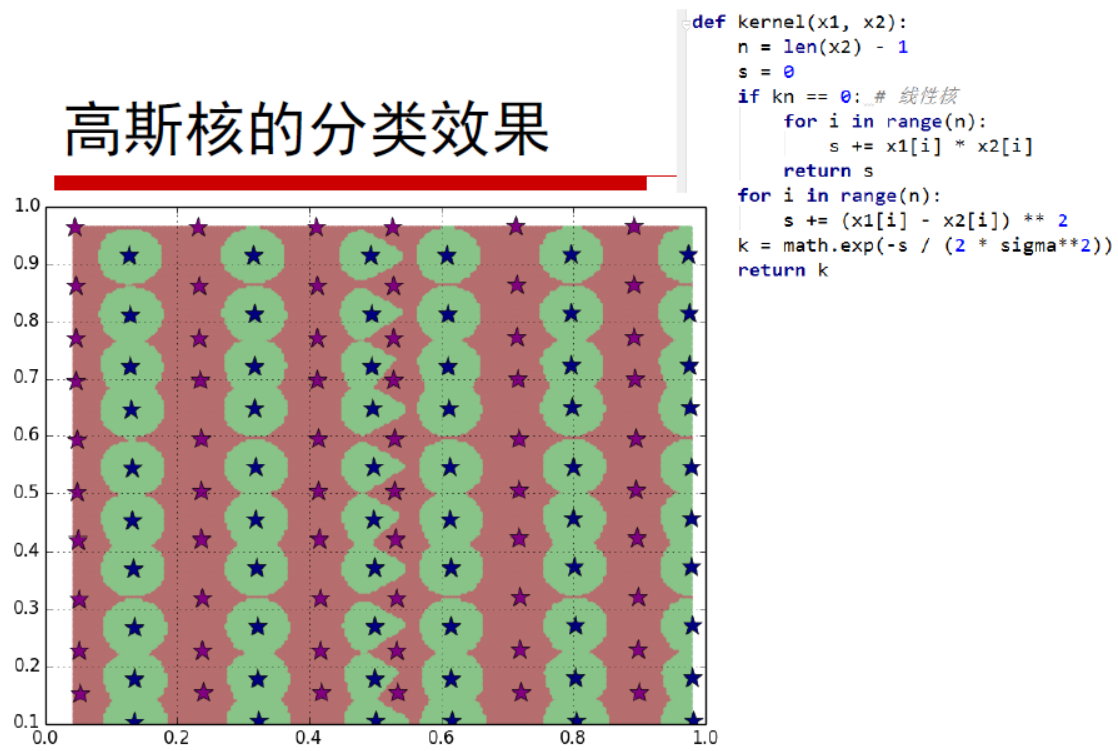
\includegraphics[height=10cm,width=14.5cm]{result_gussian_kernel_function.png}
								\renewcommand{\figurename}{Fig} % set picture title starting with Fig or 图
								\caption{gussian kernel function}
							\end{figure}							
						\end{enumerate}
					
					\item kernel function in svm
					
						选定核 $K(x_i,x_j)$ 后, 原问题变成
							\begin{align}
								\min\limits_{\alpha} \quad & \frac{1}{2}\sum_{i=1}^{n}\sum_{j=1}^{n} \alpha_i\alpha_j y_i y_j K(x_i \cdot x_j) - \sum_{i=1}^{n}\alpha_i \\
								\text{s.t.} \quad &\sum_{i=1}^{n} \alpha_i y_i = 0\\
								&0 \leq \alpha_i \leq C, \quad i=1,2,...,n
							\end{align}
						优化问题得最优解, 核要满足 Mercer 条件, 即矩阵 $k = K(x_i, x_j), (i,j = 0,1,...,n)$ 在所有训练上半正定, 说明这个优化是凸优化, 这个条件保证了最大化间隔优化问题有唯一解.
						
						最后求得 $\alpha^*, b^*$, 那么从输入空间向特征空间隐式映射后所得到的最大间隔超平面也就出来了:
							\begin{align}
								f(x) = \sum_{i=1}^{n} \alpha^* y_i K(x_i, x_j) + b^*
							\end{align}
						且有几何间隔
							\begin{align}
								\gamma = \frac{1}{\parallel w^* \parallel} = \left( \sum_{i\in\text{support vector}} \alpha^*\right)^{\frac{1}{2}}
							\end{align}
				\end{enumerate}
			
		\section{\quad sequential minimal optimization algorithm}
			\subsection{\quad concept}
				\begin{enumerate}
					\item 用于 SVM 中系数的求解算法
					
					\item 场合: 有多个 Lagrange multiplier
					
					\item 原理: 每次只选择其中两个乘子做优化, 其他因子认为是常数.
						\begin{itemize}
							\item 将 N 个解问题, 转换成两个变量的求解问题: 并且目标函数是凸的
						\end{itemize}
				\end{enumerate}
			
			\subsection{\quad process}
				\begin{enumerate}
					\item 考察目标函数
						\begin{align}
							\min\limits_{\alpha} \quad & \frac{1}{2}\sum_{i=1}^{n}\sum_{j=1}^{n} \alpha_i\alpha_j y_i y_j (x_i \cdot x_j) - \sum_{i=1}^{n}\alpha_i \\
							\text{s.t.} \quad &\sum_{i=1}^{n} \alpha_i y_i = 0\\
							&0 \leq \alpha_i \leq C, \quad i=1,2,...,n
						\end{align}

					\item 假设 $\alpha_1$ 和 $\alpha_2$ 是变量, 其他是定值:
						\begin{align}
							\begin{split}
								\min\limits_{\alpha_1, \alpha_2} \quad &W(\alpha_1, \alpha_2)\\
									&=\frac{1}{2} \kappa_{11} \alpha_1^2 + \frac{1}{2}\kappa_{22} \alpha_2^2 + y_1 y_2 \alpha_1 \alpha_2 \kappa_{12} - (\alpha_1 + \alpha_2) \\ 
									&+ y_1 \alpha_1 \sum_{i=3}^{N}y_1 \alpha_i \kappa_{i1} + y_2\alpha_2\sum_{i=3}^{N}y_i\alpha_i\kappa_{i2}
							\end{split} \label{target_function_smo}
									\\
							\begin{split}
								\text{s.t.} \quad &\alpha_1 y_1 + \alpha_2 y_2 = - \sum_{i=3}^{N}y_i\alpha_i = \xi
							\end{split} \label{equal_alpha_restrict_smo}
							\\
							\begin{split}
								&0 \leq \alpha_i \leq C
							\end{split} \label{not_equal_alpha_restrict_smo}			
						\end{align}
						其中, $\xi$ 是常数, 目标函数中省略了不含 $\alpha_1, \alpha_2$ 的常数项
						
					\item 为了求解两个变量的二次规划问题, 首先分析约束条件, 然后在此约束条件下求极小. 
						
						由于只有两个变量, 约束可以用二维空间中的图形表示
						\begin{figure}[H]
							\label{two_variable_optimization}
							\vspace{-0.2cm}  %调整图片与上文的垂直距离
							\setlength{\abovecaptionskip}{-0.2cm}   %调整图片标题与图距离
							%\setlength{\belowcaptionskip}{-1cm}   %调整图片标题与下文距离
							\centering
							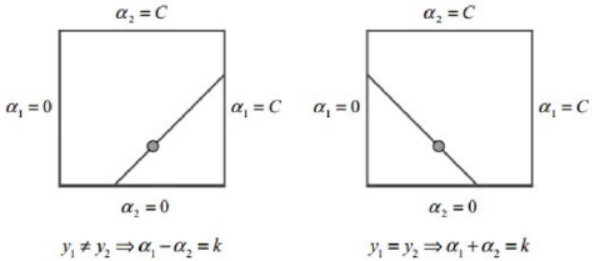
\includegraphics[scale=0.8]{two_variable_optimization.png}
							\renewcommand{\figurename}{Fig} % set picture title starting with Fig or 图
							\caption{two variable optimization}
						\end{figure}

					\item 不等式约束 \ref{not_equal_alpha_restrict_smo} 使得 	$(\alpha_1, \alpha_2)$ 在盒子 $[0, C] \times [0, C]$ 内, 等式约束 \ref{equal_alpha_restrict_smo} 使 $\alpha_1, \alpha_2$ 在平行于盒子 $[0, C] \times [0, C]$ 的对角线的直线上. 
					
						因此要求的是目标函数在一条平行于对角线的线段上的最优值. 这使得两个变量的最优化问题成为实质上的单变量的最优化问题, 不妨考虑为变量 $\alpha_2$ 的最优化问题
						
					\item 假设问题 \ref{target_function_smo} $\sim$ \ref{not_equal_alpha_restrict_smo} 的初始可行解为 $\alpha_1^{old}, \alpha_2^{old}$, 最优解为 $\alpha_1^{new}, \alpha_2^{new}$, 并且假设在沿着约束方向未经剪辑时 $\alpha_2$ 的最优解为 $\alpha_2^{new,unc}$.
					\textcolor{red}{注意:此处最优值是在图中直线上移动的}
					
					\item 综合式 \ref{equal_alpha_restrict_smo} 和 \ref{not_equal_alpha_restrict_smo} 这两个约束条件, 求取 $\alpha_2^{new}$ 的取值范围
					
					由于 $\alpha_2^{new}$ 需满足不等式约束 \ref{not_equal_alpha_restrict_smo}, 所以最优值 $\alpha_2^{new}$ 的取值范围必须满足条件
						\begin{align}
							L \leq \alpha_2^{new} \leq H
						\end{align}
					其中, L 和 H 是 $\alpha_2^{new}$ 所在的对角线段端点的界. 
						\begin{enumerate}
							\item $y_1 \neq y_2$ 时, 根据 $\alpha_1^{new} y_1 + \alpha_2^{new} y_2 = \alpha_1^{old} y_1 + \alpha_2^{old} y_2 = \xi$ 可得 $\alpha_1^{old} - \alpha_2^{old} = \xi$, 所以有
								\begin{align}
									&L = \max(0, -\xi) = \max(0, \alpha_2^{old} - \alpha_1^{old})\\
									&H = \min(C, C-\xi) = \min(C, C + \alpha_2^{old} - \alpha_1^{old})
								\end{align}
								\begin{figure}[H]	
									\vspace{-0.2cm}  %调整图片与上文的垂直距离
									\setlength{\abovecaptionskip}{-0.2cm}   %调整图片标题与图距离
									%\setlength{\belowcaptionskip}{-1cm}   %调整图片标题与下文距离
									\centering
									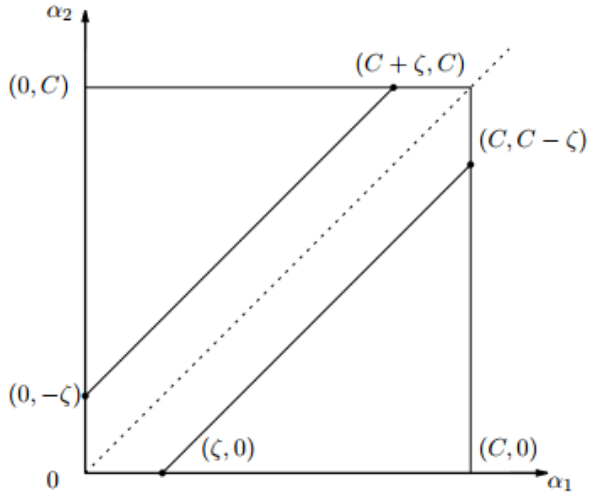
\includegraphics[scale=0.8]{y_1_not_equal_y_2_smo.png}
									\renewcommand{\figurename}{Fig} % set picture title starting with Fig or 图
									\caption{y1 not equal y2 smo}
									\label{y_1_not_equal_y_2_smo}
								\end{figure}
							
							\item $y_1 = y_2$时, 根据 $\alpha_1^{new} y_1 + \alpha_2^{new} y_2 = \alpha_1^{old} y_1 + \alpha_2^{old} y_2 = \xi$ 可得 $\alpha_1^{old} + \alpha_2^{old} = \xi$, 所以有
								\begin{align}
									&L = \max(0, \xi - C) = \max(0, \alpha_2^{old} + \alpha_1^{old} - C)\\
									&H = \min(C, \xi) = \min(C, \alpha_2^{old} + \alpha_1^{old})
								\end{align}
								\begin{figure}[H]
									\vspace{-0.2cm}  %调整图片与上文的垂直距离
									\setlength{\abovecaptionskip}{-0.2cm}   %调整图片标题与图距离
									%\setlength{\belowcaptionskip}{-1cm}   %调整图片标题与下文距离
									\centering
									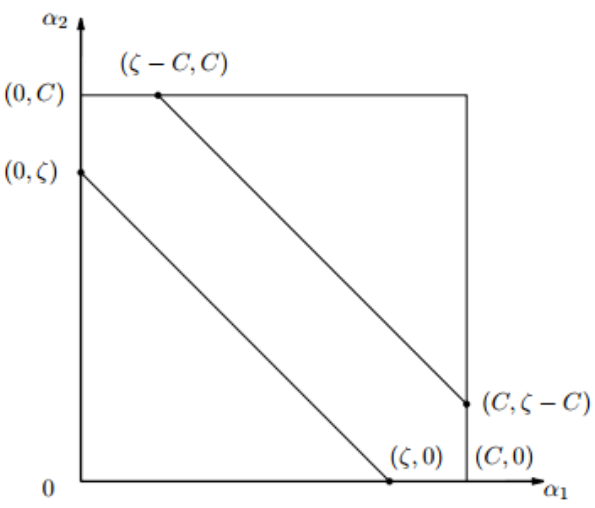
\includegraphics[scale=0.8]{y_1_equal_y_2_smo.png}
									\renewcommand{\figurename}{Fig} % set picture title starting with Fig or 图
									\caption{y1 equal y2 smo}
									\label{y_1_equal_y_2_smo}
								\end{figure}
						\end{enumerate}
					
					\item 下面首先求沿着约束方向未经剪辑即未考虑不等式约束 \ref{not_equal_alpha_restrict_smo} 时 $\alpha_2$ 的最优解 $\alpha_2^{new, unc}$; 然后再求剪辑后 $\alpha_2$ 的解 $\alpha_2^{new}$. 
					
					\textcolor{red}{以下smo此时求解 $\alpha_1$ 和 $\alpha_2$ 的迭代公式}	
					
					为叙述简单记, 记(此处 $g(x)$ 中 i 和下面 E 中所表示的 j 一致)
						\begin{align}
							g(x) = \sum_{i=1}^{N} \alpha_2 y_i K(x_i, x) + b
						\end{align}
						令
						\begin{align}
							E_i = g(x_i) - y_i = \left( \sum_{j=1}^{N} \alpha_j y_j K(x_j, x_i) + b \right) - y_i \quad i=1,2
						\end{align}
						令
						\begin{align}
							\eta = K_{11} + K_{22} - 2K{12} = \parallel \phi(x_1) - \phi(x_2) \parallel^2
						\end{align}
						$\phi(x)$ 是输入空间到特征空间的映射, $E_i, \quad i=1,2$
						
						则最优化问题 \ref{target_function_smo} $\sim$ \ref{not_equal_alpha_restrict_smo} 沿着约束方向未经剪辑时的解是
						\begin{align}
							\alpha_2^{new, unc} = \alpha_2^{old} + \frac{y_2(E_1 - E_2)}{\eta}
						\end{align}
						经剪辑后 $\alpha_2$ 的解是
						\begin{align}
							\alpha_2^{new} = \left\{
								\begin{matrix}
									&H, &\alpha_2^{new, unc} > H\\
									&\alpha_2^{new, unc}, &L\leq \alpha_2^{new, unc} \leq H\\
									&L, &\alpha_2^{new, unc} < L
								\end{matrix}
							\right.
						\end{align}
						由 $\alpha_2^{new}$ 求得 $\alpha_1^{new}$ 是
							\begin{align}
								\alpha_1^{new} = \alpha_1^{old} + y_1 y_2 (\alpha_2^{old} - \alpha_2^{new})
							\end{align}
						上述公式具体证明过程看博客
						\url{https://blog.csdn.net/v_JULY_v/article/details/7624837}
						\url{https://www.cnblogs.com/jerrylead/archive/2011/03/18/1988419.html}
						\url{https://blog.csdn.net/the_lastest/article/details/78637565}
						结合李航的统计学和周志华的机器学习
					
					\item 如何选择乘子 $\alpha_1$ 和 $\alpha_2$ (参考统计学习方法, 介绍详细)
					
					SMO 算法在每个子问题中选择两个变量优化, 其中至少一个变量是违反 KKT 条件的.
						\begin{itemize}
							\item 对于 $\alpha_1$, 即第一个乘子, 可以通过3种不满足 KKT 的条件来找
							
							\item 对于第二个乘子 $\alpha_2$ 可以寻找满足条件: $\max|E_i - E_j|$ 的乘子
						\end{itemize}
					
					\item 计算 阈值 b 和 差值 $E_i$
						b在满足下述条件:
							\begin{align}
								b = \left\{
									\begin{matrix}
										&b_1 &if \ 0<\alpha_1^{new}<C\\
										&b_1 &if \ 0<\alpha_1^{new}<C\\
										&(b_1 + b_2)/2 &otherwise
									\end{matrix}
								\right.
							\end{align} 
						下更新b:
							\begin{align}
							\centering
								&b_1^{new} = b^{old} - E_1 - y_1(\alpha_1^{new} - \alpha_1^{old}) K(x_1, x_1) - y_2(\alpha_2^{new} - \alpha_2{old}) K(x_1, x_2) \\
								&b_2^{new} = b^{old} - E_2 - y_1(\alpha_1^{new} - \alpha_1^{old}) K(x_1, x_2) - y_2(\alpha_2^{new} - \alpha_2{old}) K(x_2, x_2)
							\end{align}	
						且每次更新完两个乘子的优化后, 都需要再重新计算 b, 及对应的 $E_i$ 值
						
						最后更新完所有 $\alpha_i$, y 和 b, 这样模型就出来了, 从而即可求出咱们开头提出的分类函数:
							\begin{align}
								f(x) = \sum_{i=1}^{n} \alpha_i y_i <x_i, x> + b
							\end{align}
							
					\item summary of smo algorithm step
					
						输入: 训练数据集 $T = \left\{ (x_1,y_1), (x_2,y_2),..,(x_N,y_N)\right\}$, 其中, $x_i \in \chi = \boldsymbol{R}^n, \ y_i \in \gamma={-1,+1}, \ i=1,2,...,N$, 精度$\varepsilon$
						
						输出: 近似解 $\hat{\alpha}$
						\begin{enumerate}[(1)]
							\item 取初值 $\alpha^{(0)} = 0$, 令 $k=0$
							
							\item 选取优化变量 $\alpha_1^{k}, \alpha_2^{k}$, 解析求解两个变量的最优化问题 \ref{target_function_smo} $\sim$ \ref{not_equal_alpha_restrict_smo}, 求得最优解 $\alpha_1^{k+1}, \alpha_2^{k+1}$, 更新 $\alpha$ 为 $\alpha^{(k+1)}$
								\begin{enumerate}
									\item 第一步选取一对 $\alpha_i$ 和 $\alpha_j$, 选取方法使用启发方法
									
									\item 第二步, 固定除 $\alpha_i$ 和 $\alpha_j$ 之外的其他参数, 确定 W 极值条件下的 $\alpha_i, \alpha_j$ 由 $\alpha_i$ 表示
								\end{enumerate}
							
								\textcolor{red}{detail explaintation:}
								 \begin{enumerate}
								 	\item 假定在某一次迭代中, 需要更新 $x_1, x_2$ 对应的拉格朗日乘子 $\alpha_1, \alpha_2$, 那么这个小规模的二次规划问题写为:
									 	\begin{figure}[H]
									 		\vspace{-0.2cm}  %调整图片与上文的垂直距离
									 		\setlength{\abovecaptionskip}{-0.2cm}   %调整图片标题与图距离
									 		%\setlength{\belowcaptionskip}{-1cm}   %调整图片标题与下文距离
									 		\centering
									 		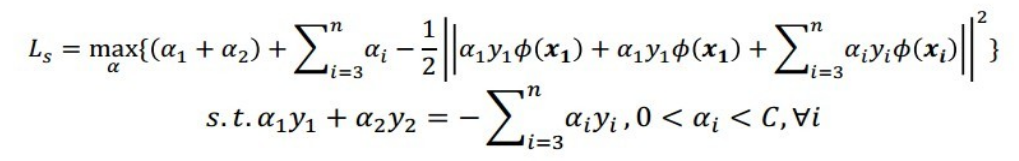
\includegraphics[scale=0.5]{update_alpha_smo_summary.png}
									 		\renewcommand{\figurename}{Fig} % set picture title starting with Fig or 图
									 		\caption{update alpha smo summary}
									 		\label{update_alpha_smo_summary}
									 	\end{figure}

									\item 那么在每次迭代中, 如何更新乘子呢? 引用\url{http://staff.ustc.edu.cn/~ketang/PPT/PRLec5.pdf}的两张ppt说明下:
										\begin{figure}[H]
											\vspace{-0.2cm}  %调整图片与上文的垂直距离
											\setlength{\abovecaptionskip}{-0.2cm}   %调整图片标题与图距离
											%\setlength{\belowcaptionskip}{-1cm}   %调整图片标题与下文距离
											\centering
											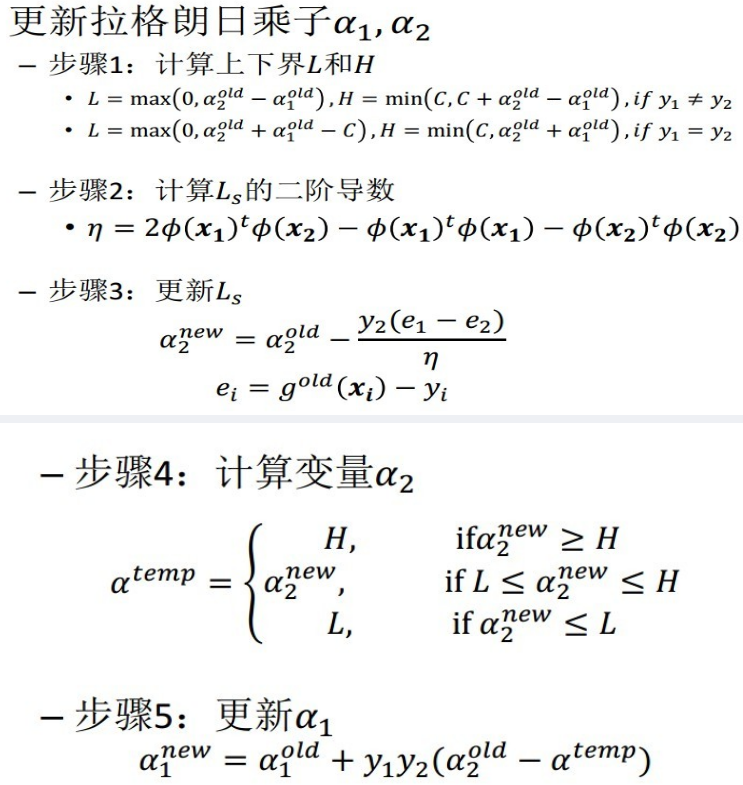
\includegraphics[scale=0.7]{detail_update_alpha_smo_summary.png}
											\renewcommand{\figurename}{Fig} % set picture title starting with Fig or 图
											\caption{detail update alpha smo summary}
											\label{detail_update_alpha_smo_summary}
										\end{figure}
									
									\item 知道了如何更新乘子, 那么选取哪些乘子进行更新呢?具体选择方法有以下两个步骤:
										\begin{itemize}
											\item step1: 先 “扫描” 所有乘子, 把第一个违反 KKT 条件的作为更新对象, 令为 $a_1$
											
											\item step2: 在所有不违反 KKT 条件的乘子中, 选择使 $|E_1 - E_2|$ 最大的 $\alpha_2$ 进行更新, 使得能最大限度增大目标函数的值 (类似于梯度下降, 此外 $E_i = \mu_i - y_i$, 而 $\boldsymbol{\mu} = \vec{w} \cdot \vec{x} - b$, 求出来的 E 代表函数 $\mu_i$ 对输入 $x_i$ 的预测值与真实输出类标记 $y_i$ 之差)
										\end{itemize}
									
									\item 每次更新完两个乘子的优化后, 都需要再重新计算 b, 及对应的 $E_i$ 值
								 \end{enumerate}
									
							\item 若在精度 $\varepsilon$ 范围内满足停机条件
								\begin{align}
									&\sum_{i=1}^{N} \alpha_i y_i = 0\\
									&0 \leq \alpha_i \leq C, \quad i =1,2,..,N\\
									&y_i \cdot g(x_i) = 
										\left\{  
											\begin{matrix}
												&\geq 1, &\{x_i | \alpha_i=0 \}\\
												&=1, &\{ x_i | 0<\alpha_i<C\}\\
												&\leq 1, &\{ x_i | \alpha_i = C\}
											\end{matrix}
										\right.
								\end{align}
								其中, 
									\begin{align}
										g(x_i) = \sum_{j=1}^{N} \alpha_j y_j K(x_j, x_i) + b
									\end{align}
								则转 (4), 否则令 $k = k + 1$, 转 (2)
								
							\item 取 $\hat{\alpha} = \alpha^{(k+1)}$
						\end{enumerate}
				\end{enumerate}
			
			与通常的分解算法比较,尽管 SMO 可能需要更多的迭代次数,但每次迭代的计算量比较小,所以该算法表现出较好的快速收敛性,且不需要存储核矩阵,也没有矩阵运算。
\end{document}